\documentclass[a4paper]{article}

% CJK support: prefer ctex, fallback to XeTeX native line breaking
\IfFileExists{ctex.sty}{
  \usepackage[fontset=fandol]{ctex}
}{
  \usepackage{fontspec}
  \XeTeXlinebreaklocale "zh"
  \XeTeXlinebreakskip = 0pt plus 1pt
  \IfFontExistsTF{Songti SC}{\setmainfont{Songti SC}}{%
    \IfFontExistsTF{Noto Serif CJK SC}{\setmainfont{Noto Serif CJK SC}}{}%
  }
  \IfFontExistsTF{Heiti SC}{\setsansfont{Heiti SC}}{%
    \IfFontExistsTF{Noto Sans CJK SC}{\setsansfont{Noto Sans CJK SC}}{}%
  }
}

% Basic packages
\usepackage{amsmath, amssymb}
\usepackage{graphicx}
\usepackage[margin=2.5cm]{geometry}
\emergencystretch=3em
\usepackage[most]{tcolorbox}
\usepackage{etoolbox}
\usepackage{listings}
\usepackage{hyperref}
\hypersetup{hidelinks,pdftitle={南京大学生成式软件工程第9讲：DeepSeek Harness (1)},pdfauthor={lecture-to-notes}}
\usepackage{booktabs}
\usepackage{subcaption}
\usepackage{float}
\usepackage{tikz}
\IfFileExists{pgfplots.sty}{
    \usepackage{pgfplots}
    \pgfplotsset{compat=1.18}
}{}

% ===== Highlight boxes =====
\newtcolorbox{knowledgebox}[1]{
    enhanced, colback=black!2!white, colframe=black!65, colbacktitle=black!65,
    coltitle=white, fonttitle=\bfseries, title=#1, attach boxed title to top left={yshift=-2mm, xshift=2mm},
    boxrule=1pt, sharp corners
}

\newtcolorbox{importantbox}[1]{
    enhanced, colback=red!3!white, colframe=red!45!black, colbacktitle=red!45!black,
    coltitle=white, fonttitle=\bfseries, title=#1, sharp corners
}

\newtcolorbox{warningbox}[1]{
    enhanced, colback=red!5!white, colframe=red!75!black, colbacktitle=red!75!black,
    coltitle=white, fonttitle=\bfseries, title=#1, sharp corners
}

% ===== Code listings =====
\lstset{
    basicstyle=\ttfamily\small,
    keywordstyle=\color{blue},
    stringstyle=\color{red!60!black},
    commentstyle=\color{green!60!black},
    breaklines=true,
    frame=single,
    numbers=left,
    numberstyle=\tiny\color{gray},
    captionpos=b,
    extendedchars=false
}

% ===== Figure provenance and unit macros =====
\newcommand{\vtag}{\protect\footnotemark}
\newcommand{\srcnote}[1]{\footnotetext{视频画面时间区间：#1。若为裁剪图，时间区间仍对应原视频画面。}}
\newcommand{\degC}{\ensuremath{^{\circ}\mathrm{C}}}
\newcommand{\um}{\ensuremath{\mu\mathrm{m}}}
\newcommand{\nm}{\ensuremath{\mathrm{nm}}}
\newcommand{\angstrom}{\ensuremath{\text{\AA}}}

% ===== Front-page metadata =====
\newcommand{\notetitle}{DeepSeek Harness (1)}
\newcommand{\notesubtitle}{南京大学生成式软件工程 · 第 9 讲}
\newcommand{\noteauthors}{中文课程讲义 · lecture-to-notes}
\newcommand{\notedate}{2026 年 10 月 20 日}
\newcommand{\videochannel}{蒋炎岩主讲 / 绿导师原谅你了上传}
\newcommand{\videopublishdate}{20261020}
\newcommand{\videoduration}{89 分 24 秒}
\newcommand{\videourl}{https://www.bilibili.com/video/BV144nc6KEA4/}
\newcommand{\videocoverpath}{cover.jpg}

\begin{document}

% ===== Title page =====
\begin{titlepage}
\centering
{\Large 课程笔记\par}
\vspace{1.2cm}
{\huge\bfseries \notetitle\par}
\ifdefempty{\notesubtitle}{}{
\vspace{0.3cm}
{\large \notesubtitle\par}
}
\vspace{0.5cm}
{\large \noteauthors\par}
\vspace{0.3cm}
{\large \notedate\par}
\vspace{1.0cm}

\ifdefempty{\videocoverpath}{
{\small 请在生成笔记时填入视频封面图的本地路径。\par}
}{
\includegraphics[width=0.82\textwidth,height=0.40\textheight,keepaspectratio]{\videocoverpath}\par
}

\vfill
\begin{tcolorbox}[width=0.9\textwidth, colback=black!2!white, colframe=black!60, sharp corners]
\textbf{视频作者/频道}：\videochannel\par
\textbf{发布日期}：\videopublishdate\par
\textbf{视频时长}：\videoduration\par
\textbf{视频链接}：\url{\videourl}\par
\vspace{0.2cm}
\footnotesize 注：文内截图均裁剪自该视频对应时间点，仅用于个人学习记录与理解辅助。
\end{tcolorbox}
\end{titlepage}

\newpage
\tableofcontents
\newpage

\section{课程导读}

上一讲我们用大约 150 行 Python 代码构造了一个最小可运行的 Coding Agent（Mini-Agent）：只要让大语言模型在循环中不断接收上下文、发起 Bash 工具调用并读取返回输出，它甚至能够仅凭一句话提示词抓取地理信息并生成南京大学仙林校区的三维场景模型。然而，从“课堂演示能跑通的玩具原型”走向“真实世界中可持续演化、多人协同的软件产品”，中间横亘着巨大的工程鸿沟。当运行在高铁上的 Agent 遭遇网络中断、当长周期任务引发未知副作用、当竞争对手的新交互形态（如 Grok Bot）一夜之间让已经写好的 50 万行办公 Agent 代码假设崩塌时，传统的紧耦合单体架构就会陷入难以维护的泥潭。

本讲以开源项目 \textbf{DeepSeek Harness（简称 \texttt{dsh}）} 为核心剖析对象，沿着“\textbf{需求复杂性 $\to$ 架构权衡原理 $\to$ 微内核与事件溯源世界模型 $\to$ 插件生态与杀手级应用}”的逻辑主线展开：
\begin{itemize}
    \item \textbf{核心问题}：当真实世界中的网络故障、权限边界、预算限制以及剧烈的产品需求变动不断冲击最小 Agent 循环时，软件架构应当在“受限（规矩）”与“自由（解耦）”之间如何取舍，才能让 Agent 底座既保持概念极简，又能生长出开放的插件生态？
    \item \textbf{核心思路}：DeepSeek Harness 采取了“\textbf{Everything Is a Plugin（万物皆插件）}”与“\textbf{Event Sourcing（事件溯源）}”相结合的微内核总线架构。系统以只追加（append-only）的 \texttt{Session = list[Event]} 作为唯一事实源（Ground Truth），将模型上下文、对话界面和调试轨迹统一抽象为事件流上的只读投影（Projection），并通过受控的 \texttt{agent/pre-step} 拦截钩子、\texttt{Scope} 权限求交与 \texttt{Slots} 界面插槽实现插件间的安全协同。
    \item \textbf{本讲收获}：读者不仅能够从软件工程第一性原理理解 LAMP、MapReduce、Spark/Flink 到 Agent Harness 的架构演进脉络，还能掌握 DeepSeek Harness 的五条核心源码契约，并学会如何利用该架构以极薄的桥接层赋能传统大型应用（SuperApp）以及构建双向交互的生成式用户界面（GenUI）。
\end{itemize}

\begin{table}[H]
\centering
\small
\begin{tabular}{p{3.4cm}p{5.2cm}p{5.2cm}}
\toprule
\textbf{预备概念} & \textbf{在本讲中的含义} & \textbf{建议带着思考的问题} \\
\midrule
最小 Agent 循环（Agent Loop） & 模型通过 Responses / Chat API 与工具反复“一问一答”的闭环执行过程 & 当外围加上重试、恢复、权限、审计和随时改需求后，为什么不能直接把逻辑塞进主循环？ \\
本质复杂性与偶然复杂性 & Brooks（1986）提出的需求固有复杂度 vs 工具与实现方式带来的附加复杂度 & 网络中断恢复、工具非幂等副作用、多插件语义冲突，分别属于哪一类复杂性？ \\
事件溯源（Event Sourcing） & 不直接原地覆写当前状态，而是以只追加日志记录所有已发生事实，由事实折叠派生状态 & 把 \texttt{Session} 定义为 \texttt{list[Event]} 对回放、多视图切换和热插拔插件有什么决定性好处？ \\
微内核与插件生命周期（Cordis） & 宿主不内置固定业务模块，而是负责服务解析、依赖激活、作用域隔离与卸载清理 & 为什么说单纯的“万物皆进程/Actor”没有工程价值，必须配合共享的世界模型与总线协议？ \\
\bottomrule
\end{tabular}
\caption{阅读本讲内容所需的核心预备知识与思考线索}
\end{table}

\begin{table}[H]
\centering
\small
\begin{tabular}{p{2.8cm}p{4.8cm}p{6.2cm}}
\toprule
\textbf{阅读目标} & \textbf{重点阅读章节} & \textbf{你将获得的核心结论} \\
\midrule
理解为什么最小 Agent 无法直接当产品交付 & 第 2 节、第 3 节 & 剖析高铁断网、API 非幂等重试、WorkBuddy 级需求膨胀与 Grok Bot 需求突变带来的架构挑战 \\
掌握软件架构设计的权衡方法论 & 第 4 节、第 5 节 & 理解“规矩换能力、自由生生态”的平衡谱系，以及从 LAMP、MapReduce（2004）到 Spark/Flink 的假设演进 \\
吃透 DeepSeek Harness 的核心设计 & 第 6 节、第 7 节、第 8 节 & 掌握 \texttt{Session} 事件溯源、\texttt{Projection} 投影、\texttt{followup/inject/steer} 输入队列、\texttt{pre-step} 钩子与 \texttt{Creator Mode} \\
探索 AI 原生应用开发与源码实现契约 & 第 9 节、第 10 节 & 学习大型应用三步桥接法（Excalidraw 案例）、GenUI 双向通道（五子棋案例）以及源码级五条核心契约 \\
\bottomrule
\end{tabular}
\caption{不同学习目标读者的讲义阅读路径指南}
\end{table}

\section{软件工程主线回顾与多 Agent 时代的协作锁}\label{sec:review}

在进入 DeepSeek Harness 的具体架构之前，我们先将前八讲建立的生成式软件工程概念体系做一个串接。软件工程最底层的问题从未改变，但当开发主体从“单线程的人类程序员”变成“多层级并发的 Agent 军团”时，版本控制与项目管理的基础假设正在被彻底改写。

\subsection{意图、规格与实现的鸿沟及复杂性二分}

软件工程的核心矛盾，始终在于人类脑海中的\textbf{意图（Intent）}、写成文档或接口契约的\textbf{规格（Specification）}与最终落地的\textbf{代码实现（Implementation）}三者之间不可避免的鸿沟（Gap）。即便在人类严密组织的航天工程中，这一鸿沟也屡屡酿成灾难——例如课件回顾的 \textbf{1999 年美国火星气候轨道器（Mars Climate Orbiter）事故}：接口规格书中明明已经规定冲量数据统一采用公制单位（牛顿$\cdot$秒），但地面软件模块实际交付的数据仍然是英制单位（磅力$\cdot$秒），最终导致探测器在进入火星轨道时高度过低而坠毁。

\begin{figure}[H]
\centering
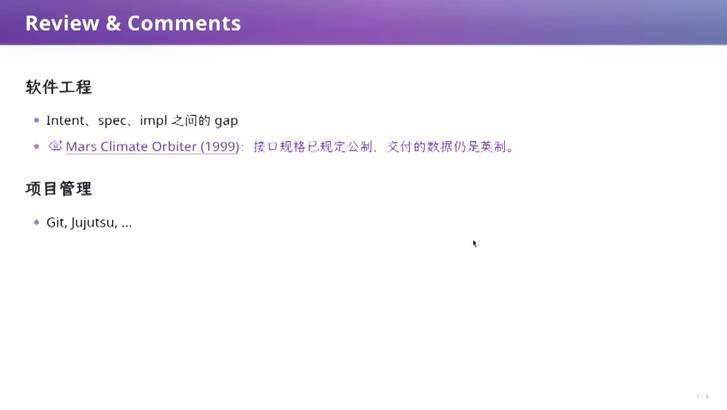
\includegraphics[width=0.84\textwidth]{figures/fig_01_review_se_git.png}
\caption{课程回顾：软件工程中意图、规格与实现之间的鸿沟（1999 年火星气候轨道器公英制单位不一致事故）以及版本控制工具演进\vtag}
\end{figure}
\srcnote{00:00:15--00:00:30}

为了弥合这一鸿沟，软件工程发展出了类型系统、形式化验证、测试驱动开发以及 CI/CD 等诸多实践范式。在评估这些范式时，弗雷德里克$\cdot$布鲁克斯（Fred Brooks）在 \textbf{1986 年经典论文《没有银弹》（No Silver Bullet）} 中提出的二分法依然是今天最犀利的判据：
\begin{enumerate}
    \item \textbf{本质复杂性（Essential Complexity）}：根植于问题域与用户需求本身的复杂性——例如现实业务规则的交织、物理网络的不可靠、跨系统状态的一致性要求。无论采用多么先进的编程语言或大模型，这部分复杂性都无法被消除。
    \item \textbf{偶然复杂性（Accidental Complexity）}：由于我们选用的开发工具、编程框架、语法样板或组织沟通方式不够理想而人为引入的复杂性。Brooks 在 1986 年指出一条定量界限：\textbf{如果软件开发中花在偶然复杂性上的工作量不到九成（90\%），那么即便一项新技术把偶然复杂性全部消除，也换不来十倍（10x）的生产力提升。}
\end{enumerate}

\begin{figure}[H]
\centering
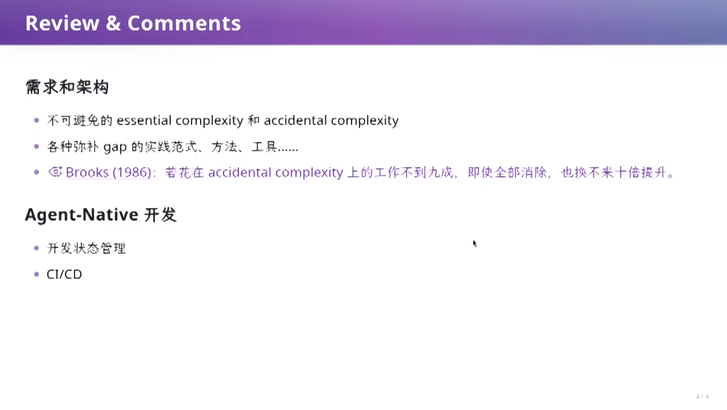
\includegraphics[width=0.84\textwidth]{figures/fig_02_review_complexity_agent.png}
\caption{课程回顾：本质复杂性与偶然复杂性的区分（Brooks 1986 银弹判据）以及 Agent-Native 开发中的外显状态管理与 CI/CD\vtag}
\end{figure}
\srcnote{00:01:45--00:02:00}

\subsection{当程序员成为 CTO：多 Agent 组织层级与代码库细粒度锁}

为什么近期 Anthropic 等前沿团队公开表示“现有的 Git 在高并发 Agent 开发下已经不够用了”？回想我们在学生时代的“古法编程”：每个学生自己就是一个单线程执行体（Single-Thread Agent），学了 C++、Python、JavaScript 后在本地单步修改代码，偶尔与一两个队友合写大作业。但在 Agent-Native 时代，一旦你拥有了成熟的 Coding Agent，你瞬间就拥有了一个现代软件公司的完整组织架构：
\begin{itemize}
    \item \textbf{人类开发者扮演 CTO / CEO}：你不再需要亲手编写每一行底层实现，而是负责全局产品方向与架构决策。
    \item \textbf{多层级 Agent 树状派发}：在你之下同时挂载着负责架构、产品、UI、前端、后端的多个主 Agent；每一个主 Agent 又会派生（Fan-out）出多个 Subagent，甚至 Subagent 还会递归创建更细粒度的执行子代理。
\end{itemize}

\begin{figure}[H]
\centering
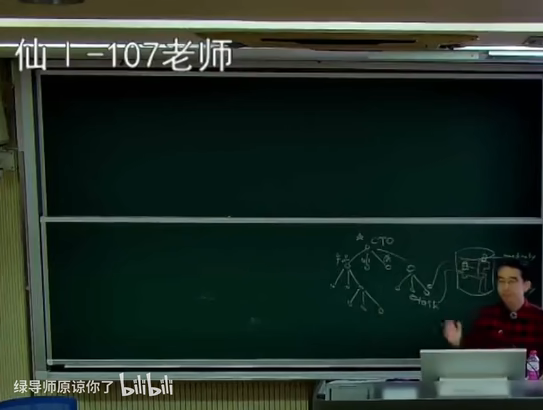
\includegraphics[width=0.72\textwidth]{figures/fig_03_board_org_locks.png}
\caption{课堂板书：CTO 统领的多层级 Agent 树状组织架构（左）与不同 Task 在代码仓库上构成的只读、写入与重构锁区域（右）\vtag}
\end{figure}
\srcnote{00:03:00--00:03:15}

如上图课堂板书所示，所有这些并发运行的 Agent 最终交付的仍然存储在同一个代码仓库（Repository）中，并经过同一条 CI/CD 流水线部署上线。从第一性原理（First Principle）出发，任何一个子代理领到的具体任务（Task），都必然对应着代码仓库中某一个子系统或模块集合的访问范围。如果继续沿用传统 Git 的粗粒度分支合并，几十个 Agent 同时提交代码必然引发灾难性的合并冲突。因此，未来的 Agent-Native 版本控制需要在代码库上引入带语义的\textbf{区域锁机制}：
\begin{enumerate}
    \item \textbf{只读锁（Read-only Lock）}：仅分析代码结构、回答问题或读取接口定义，完全可并发。
    \item \textbf{局部写锁 / 微小修复锁（Minor Fix / Write Lock）}：虽然修改了某个模块的实现代码，但承诺不改变对外接口契约、不产生破坏性变更（No Breaking Change）。只要两个小修复任务触碰的模块互不相交，系统就允许它们并行推进。
    \item \textbf{重构锁（Refactor Lock）}：涉及跨模块签名变更或核心子系统重写，需要更大范围的排他保护或阶段性同步。
\end{enumerate}

在具体实现上，这种并发控制可以借鉴\textbf{操作系统中的悲观锁}（先声明锁定的模块边界再允许 Agent 动刀）或\textbf{数据库系统中的乐观并发控制}（允许 Agent 在沙箱分支上先乐观执行，提交时通过语义级冲突检测器做 Conflict Detection）。

\begin{knowledgebox}{从文件行冲突到模块语义锁的范式升级}
传统 Git 的合并冲突检测建立在“纯文本行（Line-based Diff）”之上，无法理解代码模块的接口契约边界。而在多 Agent 并发开发的时代，版本控制系统应当与构建测试及静态分析深度融合：若两个 Subagent 分别持有互不相交模块的\textbf{局部写锁（承诺不破坏对外签名）}，即使它们在同一分钟内向主干提交代码，系统也可以在验证接口契约未变后安全地自动合入。
\end{knowledgebox}

\subsection{从“古法编程”到“许愿式开发”：OHDSH 开发者沙龙的启示}

概念讲得再多，如果不落到一个真实的 Agent-Native 开源项目上亲手拆解，就容易停留在表面。很多同学在接触了网上的热门工程技能包——例如通过提问对齐需求的 \texttt{Grill me}、结构化任务拆解的 \texttt{Get Shit Done} 或 \texttt{Superpowers}——之后，如果直接把它们套用到课程实验（如操作系统 Lab 1）上，往往会在半夜发现 Agent 陷入了失控状态：Skills 驱动着成群的 Subagent 疯狂派生（Fan-out），反复执行大量你根本不关心的边缘测试或冗余校验，面对未知问题时更是在原地空转。

为了让大家看清一个真正优秀的 Agent 底座是如何设计的，本讲选取了近期开源社区极具代表性的 \textbf{DeepSeek Harness（\texttt{dsh}）}。就在本讲授课前两天（2026 年 10 月 18 日），主讲教师在北京旁听了由社区开发者自发组织的 \textbf{OMDSH / OHDSH（Oh My DeepSeek Harness）首次北京线下聚会}。

\begin{figure}[H]
\centering
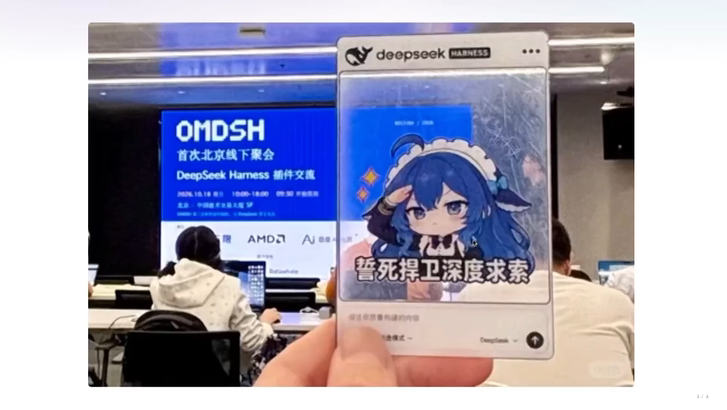
\includegraphics[width=0.82\textwidth]{figures/fig_04_ohdsh_meetup.png}
\caption{在北京举办的 DeepSeek Harness 社区首次线下插件交流聚会现场与纪念透卡\vtag}
\end{figure}
\srcnote{00:03:30--00:03:45}

这次聚会完全由民间开发者自发组织，没有一位 DeepSeek 官方员工到场，而台下许多核心插件作者正是和在座本科生同龄的年轻学生。与经历过几十年“古法编程”的老一辈程序员不同，这批年轻开发者中有不少人完全是通过对着大模型“许愿式编程（Vibe Coding）”成长起来的。主讲教师在备课期间将整套 DeepSeek Harness 编译部署到本地机器，并现场编写了多个扩展插件，全程同样没有手写一行传统业务代码，全部通过“许愿式”指令完成——只要你清楚底层架构在第一性原理上能做到什么，大模型就能帮你把它精准地落地。

\subsection{本章小结}

本节回顾了意图、规格与实现之间的鸿沟以及 Brooks 的本质/偶然复杂性判据，指出多 Agent 并发协作正在倒逼版本控制从简单的文件行合并走向带语义边界的任务锁机制，并引出了本讲的核心剖析对象——支撑“许愿式开发”与繁荣社区插件生态的 DeepSeek Harness。

\section{Agent Harness 的真实需求：从 150 行原型到工程风暴}\label{sec:requirements}

如果我们要从零构建一个类似 DeepSeek Harness 的系统，最自然的起点就是上一讲编写的 \textbf{150 行 Mini-Agent}。让我们先审视这个极简原型的能力上限，再看它是如何在真实物理世界与残酷市场竞争中被迅速击穿的。

\subsection{150 行 Mini-Agent 与南大仙林校区三维地图实验}

几乎所有现代 Agent Harness 的最内层核心，都遵循着与 150 行 Mini-Agent 完全相同的事件循环：因为大语言模型推理遵循 Responses API（或 Chat Completions API）的“一问一答”范式——无论回答模型的是人类用户，还是本地执行的工具进程，模型看到的都只是不断追加的消息序列。

\begin{figure}[H]
\centering
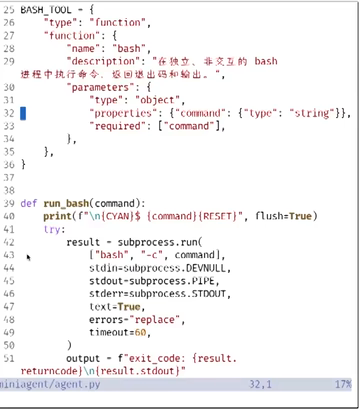
\includegraphics[width=0.52\textwidth]{figures/fig_05_miniagent_code.png}
\caption{150 行 Mini-Agent 源码中的 \texttt{BASH\_TOOL} 函数 JSON Schema 声明与带 \texttt{timeout=60} 秒限制的 \texttt{run\_bash} 执行函数\vtag}
\end{figure}
\srcnote{00:06:45--00:07:00}

如上图所示，Mini-Agent 的工具层仅仅定义了一个名为 \texttt{bash} 的函数工具（接收字符串参数 \texttt{command}），并在 Python 的 \texttt{subprocess.run(["bash", "-c", command], timeout=60, ...)} 中执行命令，将退出码 \texttt{exit\_code} 与标准输出拼接后回写给模型。这样一个简陋到极点的 Agent 究竟能干多复杂的事？

主讲教师在周五、周日搭乘高铁途中突发奇想，趁着新模型发布，只给这个 Agent 输入了字面意义上的一句话提示词：
\begin{quote}
\textbf{“生成一个相对真实的南大仙林校区 3D 图。”}
\end{quote}
令人惊讶的是，Agent 仅凭这一句话和 Bash 工具，自主编写爬虫脚本从开源地理信息库 \textbf{OpenStreetMap（OSM）} 上抓取了南京大学仙林校区的真实矢量地图数据，并生成了一个可在浏览器中交互旋转缩放的 Three.js + Vite 三维校园场景！

\begin{figure}[H]
\centering
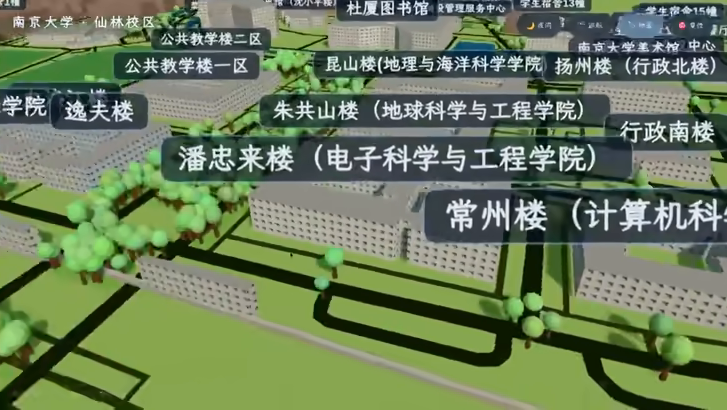
\includegraphics[width=0.84\textwidth]{figures/fig_06_nju_3d_overview.png}
\caption{一句话提示词驱动 Agent 抓取 OpenStreetMap 数据生成的南京大学仙林校区三维场景模型（含杜厦图书馆、常州楼、潘忠来楼等标注）\vtag}
\end{figure}
\srcnote{00:07:45--00:08:00}

从俯视几何轮廓（Top-Down Geometry）来看，杜厦图书馆、公共教学楼一区/二区、昆山楼、朱共山楼、潘忠来楼以及计算机系所在的常州楼的平面形状都被准确还原了。当然，One-shot 直出的第一版也暴露出模型脑补的瑕疵：
\begin{itemize}
    \item \textbf{楼层高度偏差}：计算机系所在的常州楼现实中是 10 层楼，但模型生成的三维挤压高度明显偏矮，与旁边的楼宇比例失调。
    \item \textbf{未标注区域与大门的语义误判}：OpenStreetMap 上没有建筑物的空白区块被标记为绿地，模型便在正门入口大道中央铺满了茂密的树木，甚至把校区大门牌坊也当成普通长条形楼房建模了。
\end{itemize}

\begin{figure}[H]
\centering
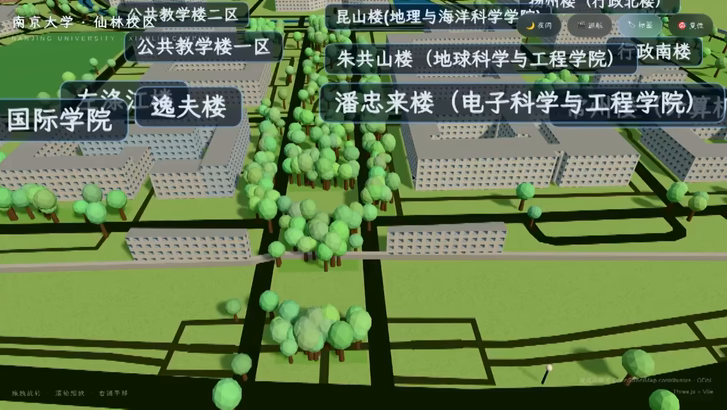
\includegraphics[width=0.84\textwidth]{figures/fig_07_nju_3d_detail.png}
\caption{南大仙林校区三维模型细节：基于 OpenStreetMap 平面轮廓自动生成的楼宇与入口绿地树木分布\vtag}
\end{figure}
\srcnote{00:09:15--00:09:30}

但这些瑕疵并不构成原理性障碍：只要在提示词中追加工作流约束——要求 Agent 先把每一块区域单独划定出来，逐一思考该区域在大学校园中的真实功能与三维形态，再分步精细建模并反复自检——哪怕多消耗 \textbf{10倍} 的 Token（“烧 Token”），就能在这个起点上迭代出可以直接拿来写“南大版 GTA”游戏的精细三维沙盒地图。

\subsection{高铁断网的暴击：API 中断、指数退避与未知副作用}

既然 150 行的 Mini-Agent 连三维校园建模都能完成，它能直接作为一个合格的软件产品发布吗？\textbf{绝对不能。}

\begin{figure}[H]
\centering
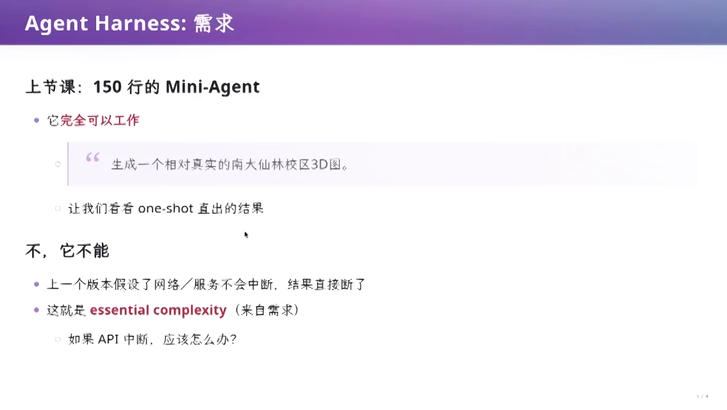
\includegraphics[width=0.84\textwidth]{figures/fig_08_harness_req_intro.png}
\caption{从 150 行玩具原型到真实产品：高铁断网暴露出“网络与服务永不中断”假设的崩塌，引出源自需求的本质复杂性\vtag}
\end{figure}
\srcnote{00:11:00--00:11:15}

在高铁上运行上述长周期建模任务时，真实物理世界给这个 150 行脚本上了一课：当列车驶入隧道或信号盲区导致网络瞬间中断时，正在等待模型 API 响应的 Python 进程直接抛出未捕获异常并崩溃退出。由于 150 行的 Mini-Agent \textbf{既没有会话持久化（Session Persistence），也没有断点恢复（Resume），更没有网络中断自动重试（Retry）机制}，此前已经跑了很长时间的上下文轨迹全部灰飞烟灭，开发者只能被迫从零重跑或者手动收拾残局。

这就是来自真实世界需求的\textbf{本质复杂性（Essential Complexity）}。一旦我们要认真设计“API 中断应该怎么办”，看似简单的重试背后立即涌现出一连串深水区工程问题：

\begin{figure}[H]
\centering
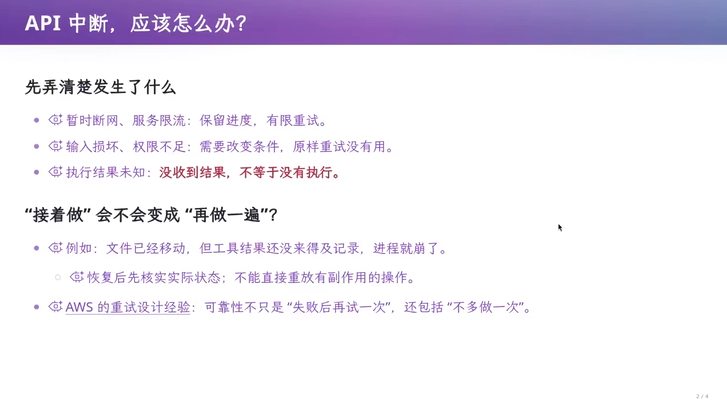
\includegraphics[width=0.84\textwidth]{figures/fig_09_api_interruption.png}
\caption{API 中断后的工程处理原则：区分故障类型、识别“未收到结果不等于未执行”的未知状态，以及遵循 AWS“不多做一次”的幂等重试设计\vtag}
\end{figure}
\srcnote{00:13:00--00:13:15}

\begin{enumerate}
    \item \textbf{网络环境差异与指数退避（Exponential Backoff）}：超时阈值（Timeout）和重试间隔设多少合适？在美国数据中心机房内网直连 OpenAI 服务，与在国内挂了 \textbf{1万} 层代理梯子访问海外 API，网络延迟与丢包分布天差地别。如果第一次请求失败后等待 1 秒重试仍然失败，下一秒大概率还是不通；因此必须引入网络协议中的指数退避策略，依次等待 \textbf{2秒}、\textbf{4秒}、\textbf{8秒}……乃至应对高铁进隧道这类持续 \textbf{2-3分钟} 的分钟级物理断网。
    \item \textbf{错误性质的精确分类}：暂时断网、HTTP 429 服务限流（Rate Limit）属于可恢复错误，应当保留进度并有限重试；而上下文超长、输入 JSON 损坏、API Key 权限不足则属于不可原样恢复的确定性错误，原样重试一万次也是白费 Token，必须改变条件或请求人工介入。
    \item \textbf{“没收到结果”绝不等于“没有执行”（未知状态与幂等性）}：这是分布式系统与 Agent 工具调用中最凶险的陷阱。好比手机端发起一笔淘宝订单或机票支付请求后瞬间断网，银行与航司服务端可能已经完成了扣款与出票提交（Commit），只是响应报文没能传回客户端；此时手机 App 绝不能直接崩溃，也不能盲目重新发起第二次扣款，而必须进入“状态未知，待同步核实”的保护态。同理，在 Agent 执行本地工具时，如果“文件已经移动（\texttt{mv}）”或“邮件已经发出”，但工具返回结果还没来得及写入会话日志进程就崩了，恢复后直接重放（Replay）最后一步就会把“接着做”变成灾难性的“再做一遍”。正如 \textbf{AWS 的重试设计经验}所总结的：\textbf{系统的可靠性不只是“失败后再试一次（At-least-once）”，更核心的是“不多做一次（Idempotency / Exactly-once semantics）”。}
\end{enumerate}

\begin{warningbox}{工程陷阱：盲目重放非幂等工具调用}
在设计 Agent 断点恢复逻辑时，绝不能把所有未闭合的工具调用（Pending Tool Call）无脑重新执行。对于纯读取类操作（如 \texttt{cat}、\texttt{grep}）可以直接重跑；但对于具有外部副作用的写操作（如修改代码、移动文件、发送请求、执行数据库迁移），恢复机制必须先探查工作区的实际状态（或要求工具提供幂等键），确认上一次操作是否已经生效。
\end{warningbox}

\subsection{需求爆炸与被真实世界包围的最小循环}

解决了网络中断与恢复，是不是就够了？远远不够。当你真的要把 Agent 做成一个面向普通用户的商业级产品——比如老板要求你对标市面上最火的办公智能体 \textbf{WorkBuddy} 写一份完整的产品需求规格说明书（SRS）——需求列表会立刻发生指数级爆炸：

\begin{figure}[H]
\centering
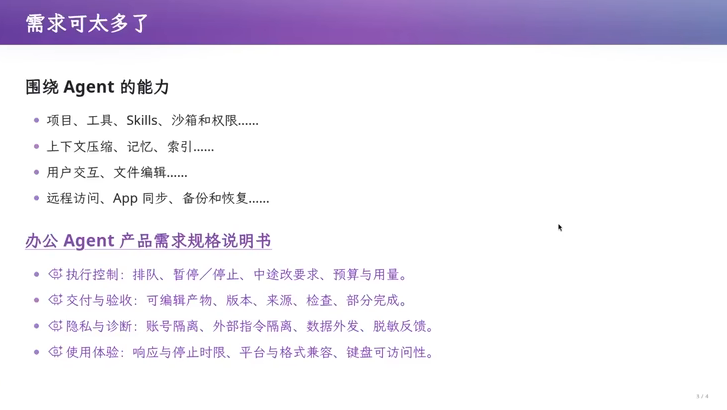
\includegraphics[width=0.84\textwidth]{figures/fig_10_requirements_explosion.png}
\caption{围绕 Agent 产品的全方位需求膨胀：从多项目工作区、Skills、沙箱权限到办公 Agent 产品需求规格说明书的四大维度\vtag}
\end{figure}
\srcnote{00:14:45--00:15:00}

主讲教师现场展示了让 AI 对标 WorkBuddy 生成的《办公 Agent 产品需求规格说明书》（涵盖把文件夹中本周项目记录整理成周报、列出延期事项并生成 Word 文件等典型场景）。仅仅翻看其中的第 12、13 条功能需求（FR12 产物管理与结果检查、FR13 历史检索与任务复用），就能感受到真实产品的繁琐程度：

\begin{figure}[H]
\centering

\includegraphics[width=0.84\textwidth]{figures/fig_11_office_agent_srs.png}
\caption{对标 WorkBuddy 生成的《办公 Agent 产品需求规格说明书》节选：重试上限、产物版本保护、必检项核对与历史任务隔离约束\vtag}
\end{figure}
\srcnote{00:16:30--00:16:45}

\begin{itemize}
    \item \textbf{重试与熔断规则}：网络暂时失败允许自动重试，每个步骤最多自动重试 2 次并显示状态；重写或写入前必须先确定上一次是否成功；相同输入和工具结果连续 3 次没有产生进展时必须自动熔断停止并说明阻塞原因。
    \item \textbf{产物管理与结果检查（FR12）}：每个产物需记录名称、格式、保存位置、生成时间、所属任务与版本，新版本不得无提示覆盖历史版本；交付前必须检查文件非空、格式可读、数值与来源核对无误，不能仅输出一句笼统的“已检查”。
    \item \textbf{历史检索与上下文隔离（FR13）}：支持按标题、日期和状态检索历史任务；复制历史任务重跑时不得把历史执行结果直接当作新任务的实际完成结果；默认严禁把其他任务的对话资料串入当前任务，防止跨任务隐私与指令污染。
\end{itemize}

\begin{figure}[H]
\centering
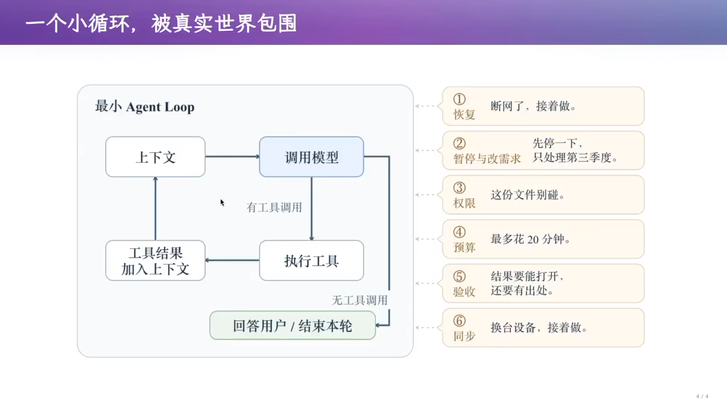
\includegraphics[width=0.84\textwidth]{figures/fig_12_loop_surrounded.png}
\caption{“一个小循环，被真实世界包围”：最小 Agent Loop 外围叠加的恢复、暂停改需求、文件权限、最多 20 分钟预算、结果验收与多端同步需求\vtag}
\end{figure}
\srcnote{00:17:30--00:17:45}

正如图 12 所直观展现的，原本清爽无比的“\textbf{上下文 $\to$ 调用模型 $\to$ 执行工具 $\to$ 工具结果加入上下文}”四步最小循环，一旦进入真实世界，外围瞬间被六大类刚性需求死死包围：（1）\textbf{恢复}（“断网了，接着做”）；（2）\textbf{暂停与中途改需求}（“先停一下，只处理第三季度”）；（3）\textbf{权限隔离}（“这份文件别碰”）；（4）\textbf{执行预算}（“最多花 \textbf{20} 分钟”）；（5）\textbf{结果验收}（“结果要能打开，还要有出处”）；（6）\textbf{跨设备同步}（“换台设备，接着做”）。如果你直接把这份冗长的需求规格说明书丢给 Coding Agent 去“一把梭”实现，由于模型具有极强的“尽快完成字面任务”的短视倾向，它必然会在核心循环里到处打满特判补丁，写出一座难以维护的代码屎山（Slop）。

\begin{importantbox}{为什么不能直接让 Coding Agent 对着长篇 SRS 一把梭？}
当前的大语言模型在没有强架构约束时，极易采取“头痛医头、脚痛医脚”的最短路径策略：把重试计数器、权限判断、超时计时器和 UI 状态回调全部硬编码进同一个 \texttt{while} 循环体中。一旦外围需求从 6 项增加到 60 项，状态转移分支就会发生组合爆炸，任何一处微小的需求调整都会牵一发而动全身。
\end{importantbox}

\subsection{杀死程序员的三次改需求：Grok Bot 冲击波与 6 月 10 日深夜的神秘提交}

比“需求繁多”更致命的挑战，是\textbf{需求的颠覆性改变}。假设你的团队已经按照上述对标 WorkBuddy 的办公 Agent 规格说明书（左侧项目树、右侧 PowerPoint View / Word View 预览栏），兢兢业业开发了 \textbf{50万} 行代码并成功上线。结果第二天早上，\textbf{Grok Bot} 突然火遍全网！

Grok Bot 带来了完全不同的交互范式：\textbf{把每个 Agent 当作有独立人格与长期记忆的“数字员工/群友”}，用户可以拉一个群让多个 Bot 协同讨论，或者交代某个 Bot 每天定时干活。这时老板冲进办公室拍板：“我们下个版本全面对标 Grok Bot！”——俗话说，“怎么杀死一个程序员？只要改三次需求就够了。”因为此前 50 万行代码所依赖的底层交互假设（以本地文件夹与文档视图为中心的工作台）彻底崩塌了！

\begin{figure}[H]
\centering
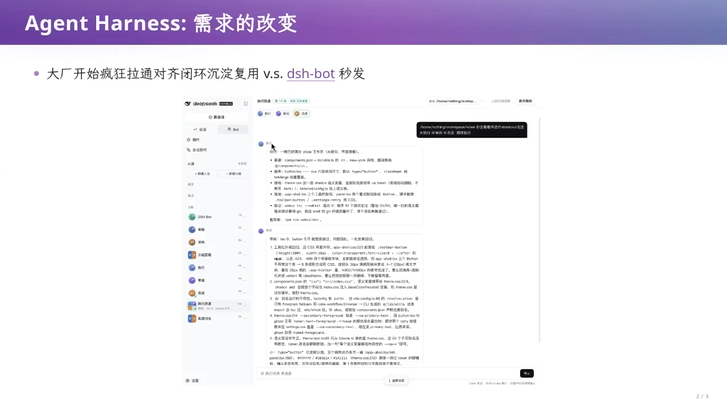
\includegraphics[width=0.84\textwidth]{figures/fig_13_req_change_dsh_bot.png}
\caption{面对 Grok Bot 需求突变：大厂被迫拉通对齐重构底座 vs. DeepSeek Harness 社区光速像素级复刻 \texttt{dsh-bot}\vtag}
\end{figure}
\srcnote{00:19:45--00:20:00}

面对这种毁灭性的范式转移，不同架构体系的反应速度截然不同：
\begin{itemize}
    \item \textbf{传统大厂重型底座的困境}：大厂为了保住极高的交付质量与确定性，往往将业务流程深度耦合在底座架构中（例如 CodeBuddy 与 WorkBuddy 共享了底层编排层）。一旦交互根基改变，大厂就不得不开启漫长的“拉通、对齐、闭环、沉淀、复用”跨部门重构周期。
    \item \textbf{\texttt{dsh-bot} 的光速复刻与自定义超越}：而在 DeepSeek Harness 社区中，几乎在瞬间就有不止一位开发者发布了 \textbf{\texttt{dsh-bot}} 插件，像素级复刻了多 Bot 配置、拉群聊天、群头像等全套体验。更关键的是，商业产品（如 Grok Bot）为了照顾 \textbf{99\%} 不懂提示词工程的普通用户，往往封闭了底层配置；而在 \texttt{dsh-bot} 上，懂行的程序员可以随时把 \texttt{config.yaml} 和系统提示词拿出来自由修改，甚至顺手 Vibe 出一个“CEO 视角多部门树状管理驾驶舱”来给自己提供情绪价值。
\end{itemize}

为什么 DeepSeek Harness 能拥有如此惊人的演进弹性？让我们把时间拨回到 \textbf{2026年} 6 月 10 日晚上 22:57（近 23:00）——当时主流产品还是 Claude Code、OpenCode、Trae 和 CodeBuddy（WorkBuddy 尚未问世），DeepSeek 内部一个神秘的仓库悄然创建了它的前两条 Git 提交：

\begin{figure}[H]
\centering
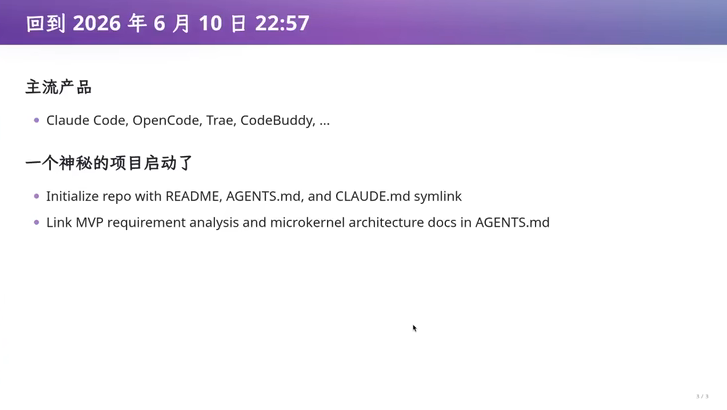
\includegraphics[width=0.84\textwidth]{figures/fig_14_june10_first_commit.png}
\caption{回到 2026 年 6 月 10 日 22:57：DeepSeek Harness 仓库启动时的前两条提交，从第一天起就确立了微内核（Microkernel）架构路线\vtag}
\end{figure}
\srcnote{00:22:45--00:23:00}

\begin{enumerate}
    \item \texttt{Initialize repo with README, AGENTS.md, and CLAUDE.md symlink}（顺带一提，当时为了兼容不同 Agent 读取项目说明的习惯，还不得不建一个 \texttt{CLAUDE.md} 软链接指向 \texttt{AGENTS.md}，这也是多 Agent 工具碎片化带来的典型偶然复杂性）。
    \item \texttt{Link MVP requirement analysis and microkernel architecture docs in AGENTS.md}。
\end{enumerate}
注意第二条提交的关键词：\textbf{\texttt{microkernel architecture}（微内核架构）}。从 6 月 10 日深夜写下第一行文档的那一刻起，设计者的目标就不是堆砌一个固定功能的 Coding Agent 应用，而是要造一艘\textbf{像操作系统一样只提供微内核与扩展协议的“航空母舰”}。

\subsection{本章小结}

本节通过 150 行 Mini-Agent 生成南大仙林校区三维地图的惊艳表现与高铁断网崩溃的强烈反差，揭示了真实世界中 API 故障分类、指数退避、非幂等副作用核实、WorkBuddy 级需求膨胀以及 Grok Bot 式需求突变的严峻挑战，说明了为什么 DeepSeek Harness 从诞生第一天起就选择了微内核架构路线。

\section{架构的经济学：规矩、自由与假设的有效期}\label{sec:architecture}

为什么面对同一个 Agent 产品需求，有的架构在需求变更时寸步难行，有的架构却能长出繁荣的生态？这需要我们回到软件工程中关于“\textbf{架构（Architecture）}”的基本理论。

\subsection{架构没有免费的午餐：“受限”与“自由”的平衡谱系}

架构的本质，是在\textbf{“受限（规矩）”与“自由”之间达成平衡}。计算机科学中没有免费的午餐（No Free Lunch）：当你选择工作在某一种架构之下时，你必然牺牲了一部分底层表达自由，以此换取基础设施为你提供的解耦、复用与系统级保障。

\begin{figure}[H]
\centering
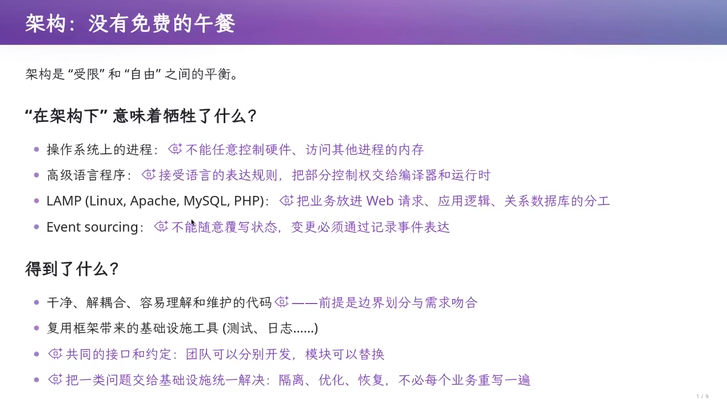
\includegraphics[width=0.84\textwidth]{figures/fig_15_arch_no_free_lunch.png}
\caption{架构没有免费的午餐：剖析操作系统进程、高级语言、LAMP 架构与 Event Sourcing 在“牺牲了什么”与“得到了什么”之间的权衡\vtag}
\end{figure}
\srcnote{00:24:15--00:24:30}

我们可以沿着计算机系统的层次结构，清晰地梳理出这一“受限换能力”的谱系：

\begin{table}[H]
\centering
\small
\begin{tabular}{p{3.0cm}p{5.2cm}p{5.6cm}}
\toprule
\textbf{架构/抽象层级} & \textbf{牺牲的自由（接受的规矩）} & \textbf{换取的系统收益（得到的午餐）} \\
\midrule
操作系统上的进程（Process） & 不能任意控制物理硬件，不能直接读写其他进程的地址空间内存 & 安全的进程隔离、虚拟内存保护、进程退出后由 OS 自动回收资源，上层可自由构建浏览器或虚拟机 \\
高级编程语言（如 C / Java / PHP） & 接受语言的语法与类型规则，把寄存器分配与部分控制权交给编译器和运行时 & 跨平台可移植性、结构化抽象与工具链支持（越接近底层的 C 越自由但也伴随内存泄漏风险） \\
LAMP 经典 Web 栈（Linux + Apache + MySQL + PHP） & 把所有业务强行塞进“Web 请求 $\to$ 无状态应用逻辑 $\to$ 关系数据库”的三层分工 & 极低的建站心智负担（如 WordPress），曾支撑互联网早期十余年繁荣 \\
事件溯源（Event Sourcing） & 严禁原地随意覆写当前状态，任何状态变更必须通过追加不可变事件（Event）来表达 & 完整的历史可追溯性（Full Persistence）、可回退至任意历史时间点、天然支持多视图派生与安全审计 \\
\bottomrule
\end{tabular}
\caption{不同软件架构层级在“牺牲自由”与“换取能力”之间的权衡对照}
\end{table}

主讲教师用一个生动的高校教务系统例子解释了 \textbf{Event Sourcing（事件溯源）} 的代价：因为当前状态完全由过去的历史事件推导（Derive）而来，首先高性能读取需要额外的投影缓存设计；其次，如果现实中遇到特殊情况——比如某位同学学分没修够，但在一个“月黑风高”的夜晚，教务员想直接在数据库里把他的状态静默改成“准予毕业”——在传统 CRUD 数据库里只需一条 \texttt{UPDATE} 语句且死无对证；但在 Event Sourcing 架构下，你不得不专门定义一种叫“强行毕业”的特殊事件并追加到持久化历史（Persistent History）中，而谁在什么时间提交（Commit）了这个事件会被永久审计留痕，再也没法用“不知道当年系统怎么搞错了”来搪塞。

\subsection{板书推演：紧耦合业务架构 vs. 过度自由的 Actor 模型}

理解了“受限与自由”的谱系后，我们来看课堂板书上对 Agent 系统架构设计的两种极端推演：

\begin{figure}[H]
\centering
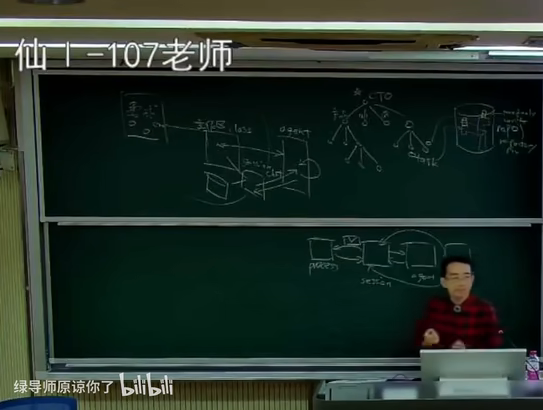
\includegraphics[width=0.72\textwidth]{figures/fig_16_board_arch_spectrum.png}
\caption{课堂板书：面向具体需求硬编码的紧耦合业务架构（左上）与完全无约束的进程消息传递 Actor 模型（右下）对比\vtag}
\end{figure}
\srcnote{00:27:00--00:27:15}

\begin{enumerate}
    \item \textbf{极端一：紧耦合的面向需求架构（板书左上方）}。当你把一份包含“工作区（Workspace）”、“会话（Session）”、“画布（Canvas）”的产品需求文档直接交给 Agent 或传统架构师时，最自然的做法就是按名词建类：写一个 \texttt{Workspace} 类，里面关联 \texttt{Session} 对象，\texttt{Session} 通过特定队列 API 向 \texttt{Agent} 发送聊天消息，\texttt{Agent} 把结果写回数据库。
    \begin{itemize}
        \item \textbf{好处}：模块边界和接口在第一天就框死了，你可以立刻启动十几个 Subagent 并行把代码堆出来，短期交付极快。
        \item \textbf{代价}：架构把当前版本的业务假设死死焊在了代码结构里。一旦明天出现 Grok Bot 或多人群聊需求，旧边界与新需求不匹配，就会到处发生\textbf{抽象泄漏（Leaky Abstraction）}，最终系统彻底腐化。
    \end{itemize}
    \item \textbf{极端二：完全自由的无约束消息模型（板书右下方）}。如果为了追求极致解耦，我们走向另一个极端——宣布“万物皆进程（Process / Actor）”，把 Workspace、Session、Agent、UI 全部拆成独立进程，规定它们内部封装私有状态（Private State），彼此之间只能通过收发消息（Message Passing）或远程过程调用（RPC）通信。
    \begin{itemize}
        \item \textbf{好处}：概念上干净到了极点，理论上可以模拟宇宙间任何软件系统。
        \item \textbf{代价}：\textbf{“太自由了等于没有架构！”}因为任何单体程序只要把函数调用替换成 RPC 就能变成这副模样。如果架构不规定“什么时候发什么格式的消息”、“状态以谁为准”、“冲突如何裁决”，开发者在写一个具体功能时依然面临无穷大的协调自由度，这样的“万能架构”在工程上毫无用处。
    \end{itemize}
\end{enumerate}

\begin{importantbox}{架构设计的核心定律}
\begin{itemize}
    \item \textbf{过于受限的架构}：在需求稳定时开发效率最高，但当底层假设改变时会因严重的抽象泄漏而成为创新的阻力。
    \item \textbf{过于自由的架构}：由于缺乏领域特定的协作规矩与共享世界模型，无法替开发者分担任何实质性的系统复杂性。
    \item \textbf{优秀的微内核架构}：必须在“完全无约束的 Actor 消息传递”之上，針對目标领域（如大模型 Agent）提炼出一套\textbf{最小但强约束的共享事实模型与扩展点协议}。
\end{itemize}
\end{importantbox}

\subsection{架构假设的有效期与 AI 产业超级加速器}

没有任何一套架构可以永恒统治世界，因为\textbf{每一套架构都建立在特定的历史与技术假设之上，而假设是有有效期的}。

以前文提到的 LAMP 架构（Linux + Apache + MySQL + PHP）为例：当互联网应用还处于单机或小规模服务器即可承载的阶段时，“PHP 是世界上最好的语言”并非一句玩笑，WordPress 等 LAMP 应用以极低的开发成本统治了 Web 世界十几年。然而，当移动互联网浪潮袭来，你的系统需要同时服务 \textbf{1亿} 乃至 \textbf{10亿} 用户时，“单机关系数据库能扛住所有读写”的底层假设彻底崩塌：从 Web 服务器到 MySQL 每一个节点都成了瓶颈；为了给数据库分库分表、引入分布式缓存与微服务拆分，原本干净的 LAMP 抽象泄漏得体无完肤，最终不得不演进到云原生分布式架构。

\begin{figure}[H]
\centering
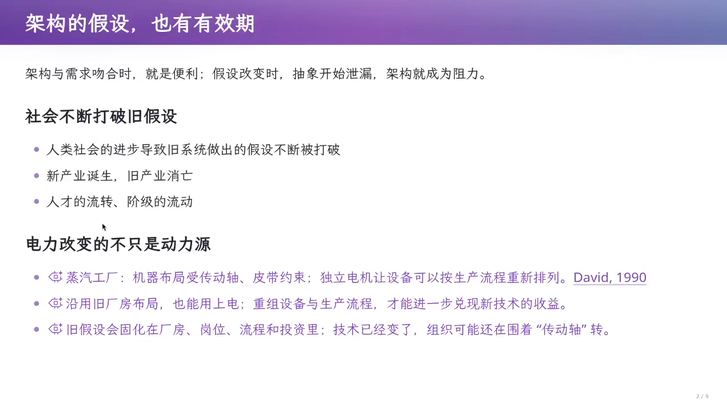
\includegraphics[width=0.84\textwidth]{figures/fig_17_arch_assumptions_expire.png}
\caption{架构假设的有效期：人类社会与技术进步不断打破旧假设，类比从蒸汽工厂集中传动轴到独立电动机流水线重组的历程（David, 1990）\vtag}
\end{figure}
\srcnote{00:31:45--00:32:00}

这种“打破旧假设、重构系统架构”的过程，在人类产业史上曾反复上演。经济史学家保罗$\cdot$大卫（Paul David）在 \textbf{1990 年的经典研究}中考察了工业革命从\textbf{蒸汽机向电力驱动}的漫长转型：
\begin{itemize}
    \item 在蒸汽工厂时代，动力来自中央蒸汽机，整座厂房的机器布局必须围绕着沉重的中央传动轴（Line Shaft）和皮带轮密集排列。
    \item 当电动机刚发明时，许多工厂只是把中央蒸汽机换成了中央大电机，继续沿用旧厂房的传动轴布局，结果生产率提升十分有限。
    \item 直到新一代工厂彻底打破“围绕中央传动轴布局”的旧假设，给每一台生产设备配备独立的小电机，并\textbf{按照物料生产流程（Workflow）重新排列整座车间与组织岗位}，电气化革命的十倍红利才真正爆发出来。
\end{itemize}

\begin{figure}[H]
\centering
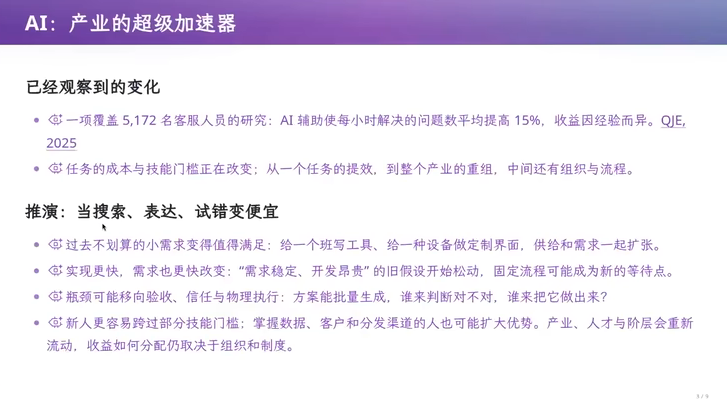
\includegraphics[width=0.84\textwidth]{figures/fig_18_ai_super_accelerator.png}
\caption{AI 作为产业的超级加速器：QJE 2025 实证研究（5,172 名客服效率提升 15\%）与“搜索、表达、试错变便宜”后的产业组织推演\vtag}
\end{figure}
\srcnote{00:33:00--00:33:15}

今天，大语言模型与生成式 AI 正在充当整个社会的\textbf{产业超级加速器}。课件引用了发表于经济学顶刊 \textbf{QJE（2025）} 的一项覆盖 \textbf{5,172} 名客服人员的实证研究：仅引入早期 AI 辅助工具，就使每小时解决的问题数平均提高了 \textbf{15\%}，且新人的技能跨越尤为明显。当我们进一步推演——当软件开发中“搜索方案、表达代码、快速试错”的边际成本坍缩到接近零时，过去支撑重型软件工程的旧假设（“需求相对稳定、写代码极其昂贵，因此必须先花三个月拉通写死规格说明书”）正在全面松动：
\begin{enumerate}
    \item \textbf{长尾微需求爆发}：过去因为开发成本太高而不划算的小需求（例如专门给一个班级写一套工具、给一种特定科研工作流做定制界面）变得值得随时满足，供给与需求同步扩张。
    \item \textbf{固定流程成为新瓶颈}：实现变得极快，需求也随之极快改变，传统的重型审批与固定排期流程反而成为最大的等待点；系统的真正瓶颈转移到了\textbf{结果验收、安全信任与物理执行}。
\end{enumerate}

\subsection{本章小结}

本节剖析了软件架构在“受限”与“自由”之间的经济学权衡，通过 LAMP 突破 1 亿～10 亿用户瓶颈与 1990 年蒸汽传动轴向独立电机转型的历史类比，阐明了“架构假设皆有有效期”，并指出 AI 带来的试错成本坍缩正在呼唤面向快速演进的新一代微内核架构。

\section{历史镜鉴：从 MapReduce 到 Spark 与 Flink 的架构演进}\label{sec:mapreduce}

为了更具体地理解“如何通过恰当的编程模型限制，换取底层基础设施的强大能力”，以及“当业务需求突破该限制时架构又该如何演进”，主讲教师带领大家精读了分布式系统历史上最具代表性的经典案例——\textbf{MapReduce} 及其后续向 \textbf{Spark} 与 \textbf{Flink} 的演进。

\subsection{OSDI 2004 MapReduce：用受限的 \texttt{map/reduce} 换取 2000 台机器的容错集群}

把目光投向 \textbf{2004年}（课堂口误先提到 \textbf{2010年} 后随即更正为 \textbf{2004年}），Google 的杰夫$\cdot$迪恩（Jeffrey Dean）与桑杰$\cdot$格玛瓦特（Sanjay Ghemawat）发表了改变整个大数据时代的里程碑论文 \textit{MapReduce: Simplified Data Processing on Large Clusters}。当时 Google 面临的核心痛点是：当你需要用成百上千台普通商用服务器（Commodity PCs）对全互联网网页建立倒排索引时，“单台机器是可靠的”这一在个人电脑大作业和单机 LAMP 时代天经地义的基本假设彻底失效了——在上千台机器组成的集群里，几乎每一刻都有机器掉线、硬盘损坏或网络分区。本科生做大作业遇到电脑蓝屏可以用“找老师求情延期”的社会工程学手段解决，但 Google 必须用系统软件的抽象层来解决。

\begin{figure}[H]
\centering
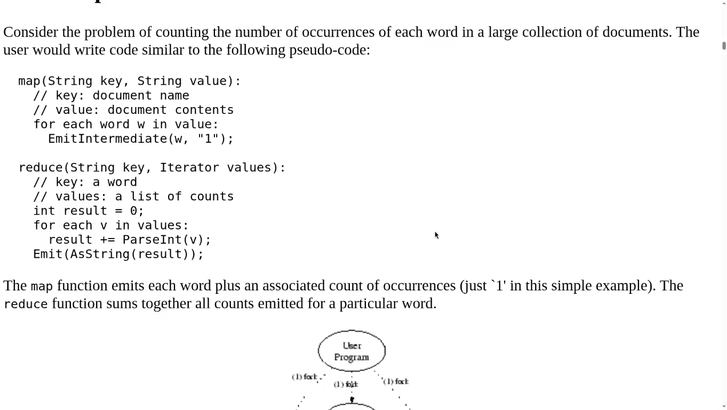
\includegraphics[width=0.84\textwidth]{figures/fig_19_mapreduce_paper_fig.png}
\caption{Jeff Dean 与 Sanjay Ghemawat 的 OSDI 2004 论文《MapReduce》中的经典词频统计（Word Count）伪代码与执行概览\vtag}
\end{figure}
\srcnote{00:34:45--00:35:00}

MapReduce 做出了一个极其经典的架构取舍：\textbf{禁止程序员编写任意结构的分布式通信与共享内存代码，强行要求所有计算都必须表达为 \texttt{map} 与 \texttt{reduce} 两个受限的高阶函数组合。}

\begin{figure}[H]
\centering
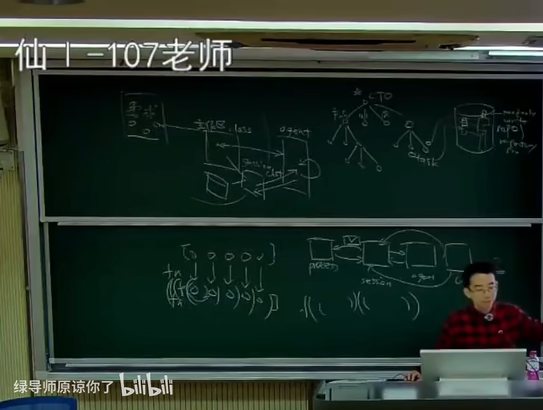
\includegraphics[width=0.72\textwidth]{figures/fig_20_board_mapreduce_tree.png}
\caption{课堂板书：函数式编程中的 \texttt{map} 列表映射（左下）与利用结合律实现并行树状归约的 \texttt{reduce} 操作（中下）\vtag}
\end{figure}
\srcnote{00:36:00--00:36:15}

结合上图课堂板书与论文中的 C++ WordCount 源码，我们可以看清这一受限模型的数学与工程本质：
\begin{enumerate}
    \item \textbf{\texttt{map} 阶段（无状态并行映射）}：给定输入列表 $[x_1, x_2, \dots, x_n]$ 与纯函数 $f$，将其逐元素映射为中间键值对列表 $[f(x_1), f(x_2), \dots, f(x_n)]$。因为每个元素的映射彼此独立，框架可以毫无顾忌地把输入切分成上万个分片（Splits），分发到不同机器上并行执行。
    \item \textbf{中间 Shuffle 与排序阶段}：框架在幕后自动把所有机器输出的相同中间 Key 的数据拉取并排序聚合在一起，程序员无需编写一行网络传输代码。
    \item \textbf{\texttt{reduce} 阶段（满足结合律的并行归约）}：对每个 Key 下的数值列表依次应用归约函数 $g$。正如板书所写，只要二元运算 $g$ 满足数学上的\textbf{结合律（Associativity）}，即 $g(g(a, b), c) = g(a, g(b, c))$，框架就可以先在局部并行归约左半部分和右半部分，再把中间结果合并！
\end{enumerate}

在 Google 内部的 C++ 实现中，程序员只需要 \texttt{\#include "mapreduce/mapreduce.h"}，继承 \texttt{Mapper} 和 \texttt{Reducer} 写几十行简单代码，并在配置对象 \texttt{MapReduceSpecification} 中声明“最多使用 \textbf{2000台} 机器（\texttt{spec.set\_machines(2000)}）、每个任务分配 100 MB 内存（\texttt{spec.set\_map\_megabytes(100)}）”，底层运行时就会自动完成数据分片、跨机调度、负载均衡与故障重算。

\subsection{抽象泄漏的边界：哪些细节 MapReduce 依然替你扛不了？}

然而，即便在 MapReduce 这样成功的受限架构下，依然存在框架无法替应用开发者屏蔽的本质复杂性：

\begin{figure}[H]
\centering
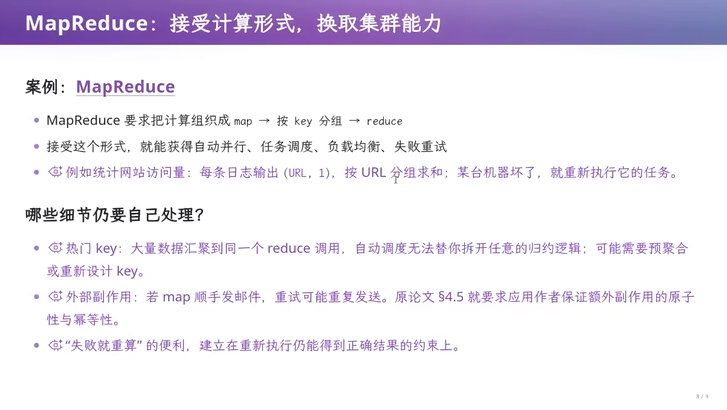
\includegraphics[width=0.84\textwidth]{figures/fig_21_mapreduce_tradeoff.png}
\caption{MapReduce 的架构取舍：接受 \texttt{map $\to$ 按 key 分组 $\to$ reduce} 换取集群容错能力，但热门 Key 倾斜与外部副作用幂等性仍需应用层自己处理\vtag}
\end{figure}
\srcnote{00:36:45--00:37:00}

\begin{itemize}
    \item \textbf{热门 Key（数据倾斜 / Hot Key Skew）}：如果全网日志统计中某一个热点 URL 占了总流量的 50\%，所有该 URL 的记录都会汇聚到同一个 \texttt{reduce} 调用节点上导致单点撑爆。如果归约逻辑不满足交换结合律，自动调度器根本无法替你拆开它，开发者必须手动设计局部预聚合（Combiner）或给 Key 加随机前缀分桶。
    \item \textbf{外部副作用与幂等性约束（原论文 §4.5）}：MapReduce“哪台机器坏了就把它的任务在另一台机器上重新跑一遍”的容错便利，完全建立在\textbf{“重新执行仍能得到相同正确结果且无额外副作用”}的强约束之上。如果程序员在 \texttt{map} 函数里顺手调接口给用户发了一封促销邮件，节点故障重试就会导致用户收到多封重复邮件！这再次印证了前文讨论 Agent API 中断重试时的同一条铁律。
\end{itemize}

\begin{knowledgebox}{结合律（Associativity）与分布式树状归约的数学联系}
为什么函数式编程如此强调纯函数（Pure Function）与结合律？当二元归约算子 $g$ 满足 $g(g(a,b),c)=g(a,g(b,c))$ 时，包含 $N$ 个元素的顺序折叠就可以在逻辑上重排为一棵深度为 $\mathcal{O}(\log N)$ 的平衡归约树。MapReduce 中的 \texttt{Combiner}（本地预归约）正是利用这一性质，在数据跨网络 Shuffle 之前先在各台 Mapper 机器上做局部折叠，从而大幅削减网络带宽开销。
\end{knowledgebox}

\subsection{当计算不再是一轮批处理：Spark 与 Flink 的范式接力}

MapReduce 辉煌了数年，但很快也撞上了它自身假设的边界：它假设所有大数据任务都是“从磁盘读取静态数据 $\to$ 一轮 Map $\to$ 一轮 Reduce $\to$ 写回磁盘”的离线批处理。当产业需求继续演进时，两代新架构应运而生：

\begin{figure}[H]
\centering
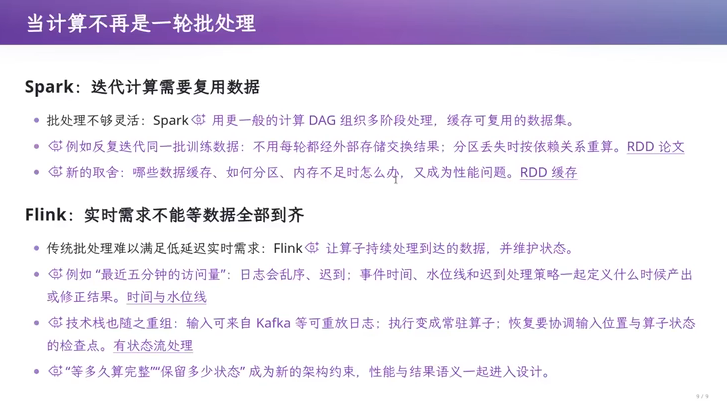
\includegraphics[width=0.84\textwidth]{figures/fig_22_spark_flink.png}
\caption{当计算不再是一轮批处理：Spark 用计算 DAG 与 RDD 内存缓存解决迭代复用，Flink 用事件时间、水位线与状态检查点解决低延迟实时流处理\vtag}
\end{figure}
\srcnote{00:37:45--00:38:00}

\begin{enumerate}
    \item \textbf{Spark（面向多轮迭代与数据复用）}：机器学习训练与图计算需要对同一批数据反复迭代数十轮。如果用 MapReduce，每一轮迭代之间都必须把中间结果落盘到分布式文件系统再重新读取，I/O 开销不可接受。Spark 将编程模型放宽为更一般的\textbf{有向无环图（DAG）}，提出\textbf{弹性分布式数据集（RDD）}，允许将可复用的数据集缓存在内存中，并在分区丢失时仅按血缘依赖关系（Lineage）局部重算。但这也带来了新的架构取舍：哪些数据该缓存、宽窄依赖如何划分、内存不足（OOM）时如何退化，成了 Spark 程序员新的调优负担。
    \item \textbf{Flink（面向低延迟实时流处理）}：当银行风控、实时推荐等需求要求“在数据到达的毫秒级内给出结果，绝不能等全部数据到齐再批处理”时，批处理假设彻底失效。Flink 让常驻算子持续处理来自 Kafka 等可重放日志的流式数据，并引入了\textbf{事件时间（Event Time）}、\textbf{水位线（Watermark）}与\textbf{分布式有状态检查点（Stateful Checkpointing）}——这也与我们即将剖析的 Event Sourcing 及函数式响应式编程有着千丝万缕的血脉联系。
\end{enumerate}

\subsection{本章小结}

本节通过复盘 MapReduce（2004）到 Spark 与 Flink 的分布式架构演进史，展示了优秀的系统架构如何通过限制编程模型换取容错与并发能力，同时揭示了幂等性约束与假设变迁如何推动新一代架构的诞生。这一历史镜鉴为我们理解 DeepSeek Harness 的设计哲学铺平了道路。

\section{DeepSeek Harness 的第一性原理与世界模型}\label{sec:world-model}

看过了分布式计算如何用“受限的 \texttt{map/reduce}”驯服集群复杂性，现在我们正式回答本讲的核心命题：\textbf{如果我们要从第一性原理（First Principle）设计一个面向未来的 Agent Harness，它的微内核应该定下什么规矩、提供什么自由？}

\subsection{Everything Is a Plugin 与 Cordis 生命周期管理}

正如我们在第 2 节看到的，DeepSeek Harness 从 2026 年 6 月 10 日的第一个提交起，就把自己定位为 Agent 时代的“微内核操作系统”。操作系统最伟大的洞察在于：\textbf{内核不需要提前知道未来上面会跑什么应用}——在 Unix 诞生之初，世界上还没有图形桌面、没有 Web 浏览器、更没有 Coding Agent，但 Unix 提供了进程（Process）、文件（File）和管道（Pipe）这组正交原语，使得任何未知的应用都能在上面自由组合。

\begin{figure}[H]
\centering
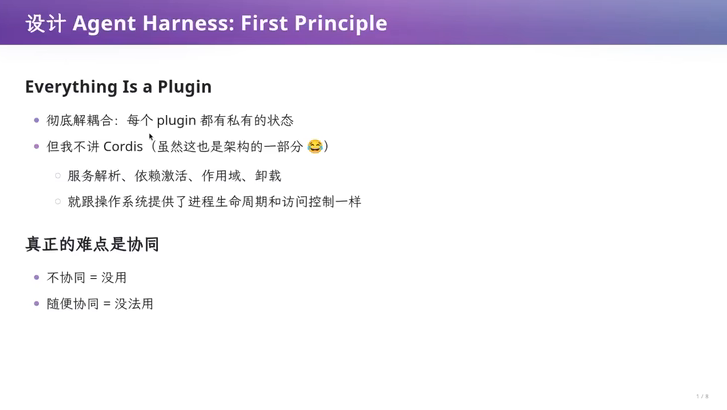
\includegraphics[width=0.84\textwidth]{figures/fig_23_first_principle_plugin.png}
\caption{设计 Agent Harness 的第一性原理：\texttt{Everything Is a Plugin}（每个插件拥有私有状态，由 Cordis 负责生命周期与作用域），而真正的难点在于插件间的协同\vtag}
\end{figure}
\srcnote{00:39:45--00:40:00}

基于这一思想，DeepSeek Harness 确立的第一性原理是 \textbf{\texttt{Everything Is a Plugin}（万物皆插件）}：
\begin{itemize}
    \item \textbf{彻底解耦合与无特权内核}：系统中没有任何写死的“特权业务内核”，甚至连大模型调用、Bash 工具、会话存储和 Web 聊天界面本身，全都是平等挂载的插件。每个插件将绝大多数业务状态（Private State）封装在自己内部。
    \item \textbf{Cordis 提供进程级资源回收保障}：DeepSeek 在开源 Harness 之前曾专门发表过一篇关于插件框架 \textbf{Cordis} 的论文（内含大量形式化公式，本讲略过其数学细节而聚焦工程作用）。Cordis 扮演的角色，恰恰相当于操作系统中的进程管理器：它负责插件的\textbf{服务解析、依赖激活、作用域（Scope）隔离以及动态加载/卸载（Load / Unload）}。
    \item \textbf{自动清理副作用（Side Effects）}：就像同学们写 OJ 算法题时从来不手动 \texttt{free} 内存，因为大家都默认“进程退出时操作系统会自动回收它持有的所有内存和文件描述符”；Cordis 将这一保障带入了插件开发——当一个插件声明了它的依赖并向系统注册了事件监听器、工具或 UI 组件后，一旦该插件在运行时被卸载（Unload），Cordis 会自动回收该插件产生的所有副作用（Effects），确保动态热插拔不会把宿主环境搞脏。
\end{itemize}

然而，正如第 4 节板书所警示的：\textbf{如果仅仅有 Cordis 的插件隔离，那它还只是一个进程内（In-process）的 Actor 模型。真正的难点在于“协同”——不协同等于没用，随便发消息协同又会乱成一团、没法用！}

\subsection{构建 Agent Harness 的“世界模型”：\texttt{Session = list[Event]} 与 1494 年的复式记账}

为了让互不相识的插件能够井然有序地协同，DeepSeek Harness 在 Cordis 插件底座之上，专门围绕大语言模型 Agent 定义了一套极简而强大的\textbf{共享“世界模型（World Model）”}。

\begin{figure}[H]
\centering
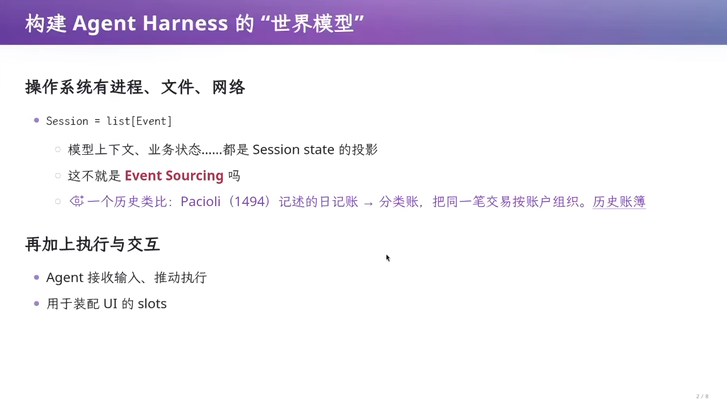
\includegraphics[width=0.84\textwidth]{figures/fig_24_world_model_event_sourcing.png}
\caption{构建 Agent Harness 的世界模型：将 \texttt{Session = list[Event]} 作为唯一事实源，模型上下文与业务状态皆为事件流的投影（类比 Pacioli 1494 年复式记账法）\vtag}
\end{figure}
\srcnote{00:42:15--00:42:30}

如果说操作系统的世界模型由“进程、文件、网络”构成，那么 DeepSeek Harness 的世界模型则由三大核心抽象构成：
\begin{enumerate}
    \item \textbf{\texttt{Session = list[Event]}（只追加的事件流是唯一事实源）}：在一个 Agent 会话中，真正被持久化存储的\textbf{不是}最终拼接好的模型 Prompt，也\textbf{不是}当前聊天窗口里的 DOM 状态，而是一条只追加（Append-only）的\textbf{事件日志（Event Log）}。无论是用户输入了一句话、模型吐出了一段推理、调用了一次 Bash 工具，还是某个插件记下了一条自定义业务记录，全部作为不可变的事实（Fact）追加到 \texttt{Session} 中。
    \item \textbf{万物皆投影（Projection）与 1494 年的历史回响}：模型推理所需的上下文消息列表（Messages）、前端展示的业务状态、Token 计费统计面板，全都不是独立存储的源数据，而是从同一个 \texttt{Session} 事件流上实时折叠计算出来的\textbf{投影（Projection / Derived State）}。主讲教师指出，这正是软件架构中的 \textbf{Event Sourcing（事件溯源）}，而它背后其实是人类在 500 多年前就发明的古老智慧——意大利数学家卢卡$\cdot$帕乔利（Luca Pacioli）在 \textbf{1494 年}系统记述的\textbf{复式记账法（Double-Entry Bookkeeping）}：商人们在交易发生时只按时间顺序往不可篡改的“日记账（Journal）”里追加每一笔原始凭证，然后再通过固定的折叠规则，把同一份日记账投影成按账户分类的“分类账（Ledger）”、资产负债表和损益表！
    \item \textbf{Agent 执行器与 UI 装配插槽（Slots）}：除了静态事实与投影，世界模型还需要驱动力与呈现层——\texttt{Agent} 负责接收输入、推动推理与工具调用循环；而 Web 前端则暴露出一组标准化的命名插槽（\texttt{slots}），允许任何插件把自己的可视化组件装配到界面的指定位置。
\end{enumerate}

\subsection{Event Bus 总线、流式 Open Entry 与无侵入扩展}

让我们结合课堂板书，看看这套世界模型在运行时是如何通过\textbf{事件总线（Event Bus）}运转的：

\begin{figure}[H]
\centering
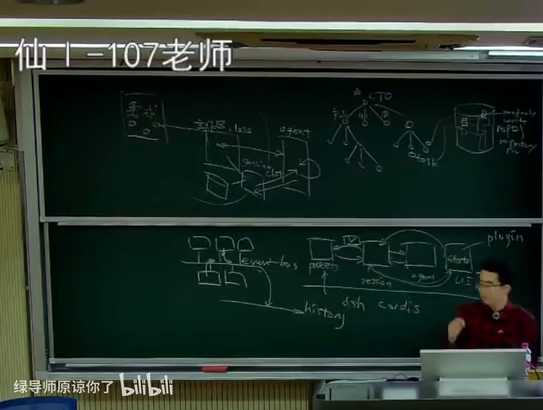
\includegraphics[width=0.72\textwidth]{figures/fig_25_board_event_bus.png}
\caption{课堂板书：在 \texttt{dsh / cordis} 之上构建共享的 \texttt{event bus} 与持久化 \texttt{history}，所有插件挂载在总线上观察事件并维护各自私有状态\vtag}
\end{figure}
\srcnote{00:45:00--00:45:15}

如上图板书所示，DeepSeek Harness 在进程空间内建立了一条受 TypeScript 强类型约束的 \textbf{\texttt{Event Bus}（事件总线）}：
\begin{itemize}
    \item \textbf{编译期类型门禁}：插件不能像在无约束 Actor 模型中那样随便往总线上乱扔任意格式的数据；每一种领域事件（如 \texttt{session/*}、\texttt{agent/*}、\texttt{capability/*}）都有严格声明的 Payload 类型，类型不匹配的代码在 TypeScript 编译阶段就会直接报错拦截。
    \item \textbf{流式 \texttt{Open Entry} 的精巧工程折中}：严格来说，持久化的 Event Sourcing 只记录已经完成提交（Committed）的不可变事实。但大模型推理是一个持续数秒到数十秒的流式吐字过程（Streaming），用户在界面上需要实时看到模型的思维链（Thinking Chain，例如课堂演示中动态跳动的 \texttt{Thinking...}）和逐字输出。为此，\texttt{dsh} 在持久化历史末尾设计了一个巧妙的\textbf{未闭合条目（Open Entry）}：在模型本轮推理尚未结束前，不断吐出的增量 Token 会实时更新这个处于 Open 状态的事件并广播到总线上，供前端 UI 实时渲染动态思维链，但它此时并不触发磁盘持久化提交；直到本轮响应完整结束，该条目才正式封口并作为一条不可变事件 Commit 到持久化日志中。
    \item \textbf{从“白板一块”长出无侵入功能}：主讲教师回忆道，DeepSeek Harness 最早期的内部测试版真的就是“白板一块”，连 Token 消耗统计和上下文占用百分比都没有。但就在内测第一天，开发者群里的同学就写出了一个 Token 与缓存命中率（Cache Hit）统计插件并挂载到了 UI 底栏插槽上。这个插件\textbf{完全不需要修改或侵入系统中的任何其他模块}——它只是静静地旁听总线上流过的模型推理完成事件，把里面的 Token 数量与 Cache Hit 数据累加到自己的私有状态里，再渲染到底栏 Slot 中。
\end{itemize}

\begin{knowledgebox}{为什么需要流式 Open Entry 这一“半持久化”过渡态？}
在纯粹的离线 Event Sourcing 系统中，只有完整结束的事务才会写入日志。但在交互式 Agent 场景下，单次大模型推理可能持续数十秒，若坚持“彻底生成完才发出唯一一条事件”，前端界面就会在几十秒内完全卡死；反之，若将每一个流式 Token delta 都作为独立事件持久化落盘，又会导致日志文件体积暴涨数千倍。因此，“内存中实时广播流式 Open Entry、完成时单次归档 Commit”是兼顾实时用户体验与持久化整洁性的经典工程折中。
\end{knowledgebox}

\subsection{本章小结}

本节揭示了 DeepSeek Harness 的两大架构支柱：一是以 Cordis 实现的 \texttt{Everything Is a Plugin} 全动态插件生命周期管理；二是以 \texttt{Session = list[Event]} 事件溯源为核心的世界模型，通过强类型 Event Bus、流式 Open Entry 与 UI Slots，让独立维护私有状态的插件实现零侵入协同。

\section{总线核心原语：Session 投影、Agent 队列与 Pre-step 钩子}\label{sec:bus-api}

很多同学在初次阅读 DeepSeek Harness 源码时会觉得它“平平无奇”，因为它的核心接口少得惊人；但主讲教师在看完这套接口后却评价其如“原子弹爆炸”般震撼——因为正是这五个极简的原语接口，精准地托起了几乎所有可能的 Agent 扩展需求。下面我们结合课件代码逐一拆解这五项核心原语。

\subsection{Session：从不可变事实到多视图投影（原语 1 \& 2）}

围绕 \texttt{Session} 的操作被严格收敛为“记录/观察事实”与“定义/读取投影”两件事：

\begin{lstlisting}[language=Java, caption={Session 事实记录观察（原语 1）与增量投影定义（原语 2）的核心 API 模式}]
// 1. 记录与观察已发生的事实 (Facts)
session.append(type, data)
ctx.on('session/event', (session, entry) => {
  // 旁听已提交到日志中的不可变事件
})

// 2. 从事实流折叠生成只读投影 (Projections)
const myProj = session.defineProjection({
  key: 'my-plugin:summary',
  initial: () => ({ count: 0 }),
  apply: (state, entry) => { /* 根据新事件增量折叠状态 */ }
})
ctx.sessionProjections.register(myProj)
const currentView = ctx.sessionProjections.stateOf(session, myProj.key)
\end{lstlisting}

这种“单一事实源 + 多路投影”的威力，在 DeepSeek Harness 官方自带的两个一级界面标签页中体现得淋漓尽致：
\begin{itemize}
    \item \textbf{模型消息投影（\texttt{session.deriveMessages()}）与人类 Chat 视图}：给大模型推理看的上下文，以及给普通用户看的清爽聊天气泡界面，都是通过过滤和折叠 \texttt{Session} 事件流派生的投影。如果你讨厌默认的聊天框样式，你完全可以把默认聊天视图设为不可见，自己写一个投影插件把同一个 \texttt{Session} 渲染成任何奇特的界面。
    \item \textbf{开发者 Trajectory（轨迹）调试视图}：在开发调试 Agent 时，我们最痛苦的就是看不清模型到底收到了什么 System Prompt、工具调用传了什么 JSON 参数、哪一步耗时最长。在 \texttt{dsh} 中，只需点击顶部的 \textbf{\texttt{Trajectory}} 标签，系统就会将\textbf{完全相同的那份 \texttt{Session} 事件流}实时投影为面向开发者的全量时间线调试器！
\end{itemize}

\begin{figure}[H]
\centering
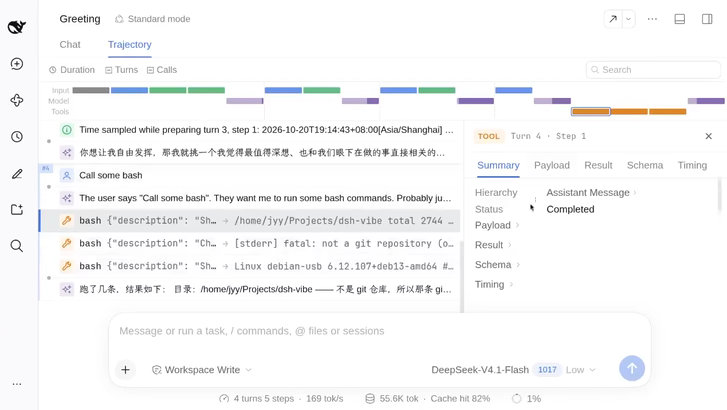
\includegraphics[width=0.84\textwidth]{figures/fig_26_dsh_trajectory_ui.png}
\caption{DeepSeek Harness 的 \texttt{Trajectory} 视图：将同一份 \texttt{Session} 事件流投影为包含时间分布条、Bash 工具调用 Payload、退出状态与实时推理速度（169 tok/s，Cache Hit 82\%）的开发者调试面板\vtag}
\end{figure}
\srcnote{00:48:45--00:49:00}

\subsection{Agent：三种输入队列语义与动态上下文贡献（原语 3 \& 4）}

当用户在模型正在思考或正在执行一连串工具调用的中途，又敲入了一句新指令时，系统应该怎么处理？在之前第 3 节的《办公 Agent 需求规格说明书》里，这曾是一个让人头疼的复杂状态机；而在 DeepSeek Harness 中，\texttt{Agent} 服务直接将其提炼为三个语义无比清晰的方法调用（原语 3），外加一个动态上下文注册接口（原语 4）：

\begin{lstlisting}[language=Java, caption={Agent 的三种输入排队/打断模式（原语 3）与动态系统提示词贡献（原语 4）}]
// 3. 向 Agent 提交输入的三种精确语义
agent.followup(message) // 排队：等当前整轮任务（Turn）全部运行完毕后，开启下一轮对话
agent.inject(message)   // 注入：放入缓冲区，在当前轮的下一个推理步（Step）边界拼入上下文，若 Agent 空闲则不主动唤醒
agent.steer(message)    // 转向/打断：紧急介入，立即中断（Abort）当前正在进行的推理或工具步骤并按新指令转向

// 4. 持续贡献动态上下文 (Dynamic System Prompt Section)
ctx.systemPrompt.context(() => ({
  text: describeCurrentState() // 每轮推理构建 Prompt 时动态求值
}))
\end{lstlisting}

\begin{table}[H]
\centering
\small
\begin{tabular}{p{2.6cm}p{3.8cm}p{3.8cm}p{3.6cm}}
\toprule
\textbf{输入原语} & \textbf{介入时机（Granularity）} & \textbf{对当前运行步骤的影响} & \textbf{典型工程场景} \\
\midrule
\texttt{agent.followup} & 轮次边界（Turn Boundary） & 不打断当前轮，等所有工具调用与最终回答结束后再排队执行 & 用户在 Codex / Claude 工作时顺手布置下一个独立任务 \\
\texttt{agent.inject} & 步骤边界（Step Boundary） & 不中断当前正在跑的命令，但在本轮下一次调用模型前把补充信息塞进上下文 & 后台监控插件把最新文件变更或传感器状态静默补充给模型 \\
\texttt{agent.steer} & 立即抢占（Immediate Preempt） & 相当于按下 \texttt{ESC} 中断当前正在跑偏的推理或工具，立即按新方向重开一步 & 发现模型理解错需求正在乱改代码，紧急喊停并纠正：“只处理第三季度！” \\
\bottomrule
\end{tabular}
\caption{Agent 三种输入提交原语的介入粒度与行为对比}
\end{table}

而原语 4（\texttt{ctx.systemPrompt.context}）则让“每一轮推理前自动把当前时区、工作目录状态、甚至外部画布选区动态注入模型 System Prompt”变得易如反掌——插件不再需要去篡改核心的 \texttt{build\_context()} 函数，只需向总线注册一个返回字符串的动态闭包即可。

\subsection{Hooks：在执行前介入决策的洋葱圈拦截（原语 5）}

如果插件只能旁听已经提交到 \texttt{Session} 里的历史事件（\texttt{session/event}），那么当模型即将执行一条危险的 \texttt{rm -rf} 命令，或者上下文即将超出窗口上限时，插件就只能“事后收尸”而无法“事前阻止”。为此，DeepSeek Harness 提供了第五项、也是整个架构中最关键的控制原语——\textbf{执行前决策钩子（\texttt{agent/pre-step}）}：

\begin{figure}[H]
\centering
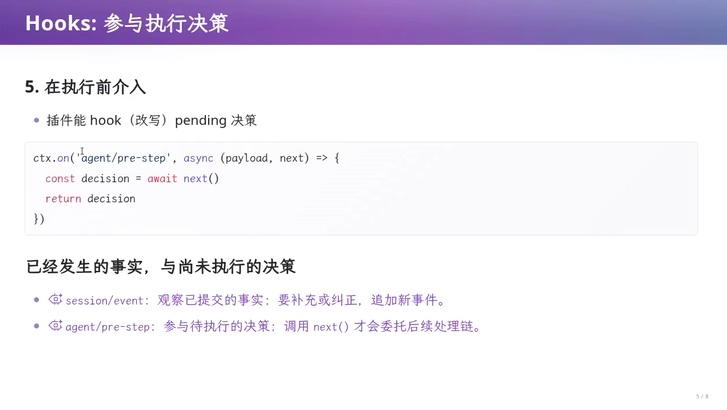
\includegraphics[width=0.84\textwidth]{figures/fig_27_session_agent_hooks_api.png}
\caption{Hooks 参与执行决策：通过 \texttt{ctx.on('agent/pre-step', ...)} 洋葱圈中间件改写或拦截尚未执行的决策，严格区分“已发生的事实”与“待执行的决策”\vtag}
\end{figure}
\srcnote{00:51:45--00:52:00}

观察上图中的代码结构：
\begin{lstlisting}[language=Java, caption={基于洋葱圈模型（Around-middleware）的 \texttt{agent/pre-step} 决策拦截钩子}]
ctx.on('agent/pre-step', async (payload, next) => {
  // 前置介入：可检查或改写即将发往模型/工具的 payload，甚至直接返回终止决策而不调用 next()
  const decision = await next()
  // 后置介入：可观察或二次包装内层插件返回的 decision
  return decision
})
\end{lstlisting}

这里体现了一个极其深刻的软件设计分野：\textbf{严格区分“已经发生的事实（Committed Facts）”与“尚未执行的决策（Pending Decisions）”}：
\begin{itemize}
    \item \textbf{\texttt{session/event}（观察已提交事实）}：采用单向广播（Emit / Serial）模式。事实一旦发生就不允许历史篡改；如果某个插件认为之前发生的事需要补充或纠正，它只能往日志末尾\textbf{追加一条新事件}。
    \item \textbf{\texttt{agent/pre-step}（参与待执行决策）}：采用类似 Koa / Express 的\textbf{洋葱圈包裹中间件（Waterfall / Around-middleware）}模式。只有当外层插件显式调用 \texttt{await next()} 时，控制权才会传递给后续处理链；外层插件既可以在调用前改写请求参数（如注入额外提示词、触发上下文压缩），也可以直接拦截并返回一个“拒绝/停止”决策，从而在单个扩展点上同时支撑起\textbf{沙箱权限审批、执行预算熔断、自动上下文压缩与安全审计}。
\end{itemize}

\subsection{总线架构全景图：少量协作接口连接各自维护状态的插件}

将上述五大原语与 Cordis 底座拼合在一起，我们就得到了 DeepSeek Harness 的完整架构蓝图：

\begin{figure}[H]
\centering
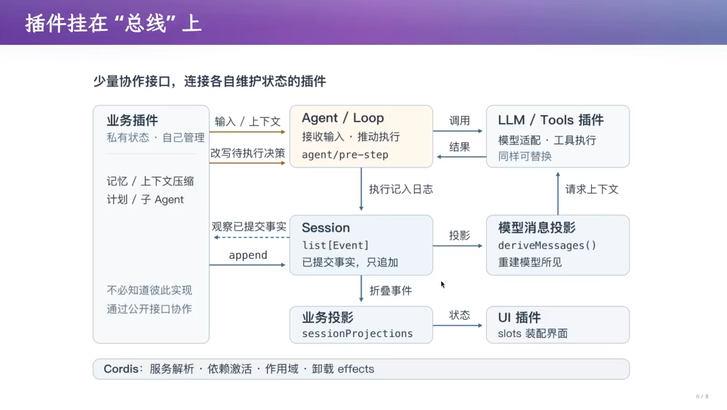
\includegraphics[width=0.84\textwidth]{figures/fig_28_plugins_on_bus_arch.png}
\caption{DeepSeek Harness 核心架构全景：业务插件、Agent/Loop、Session 事件流、模型/业务投影、LLM/Tools 插件与 UI Slots 通过极少数公开接口在总线上协同\vtag}
\end{figure}
\srcnote{00:53:00--00:53:15}

\begin{knowledgebox}{DeepSeek Harness 总线协同的数据流闭环}
如图 28 所示，系统中的所有角色各司其职且互不耦合：
\begin{enumerate}
    \item \textbf{业务插件（左侧）}：如记忆管理、上下文压缩、计划管理、子 Agent 等，各自维护私有状态；它们通过 \texttt{append} 与 \texttt{session/event} 观察已提交事实，通过 \texttt{agent/pre-step} 改写待执行决策，完全不必知道彼此的内部实现。
    \item \textbf{核心状态与执行环（中上部与右侧）}：\texttt{Agent / Loop} 驱动执行并将事实记入只追加的 \texttt{Session (list[Event])}；\texttt{Session} 向右通过 \texttt{deriveMessages()} 投影出模型所见的上下文供可替换的 \texttt{LLM / Tools 插件}调用，向下通过 \texttt{sessionProjections} 折叠出业务投影，最终交由 \texttt{UI 插件}通过 \texttt{slots} 装配成用户界面。
\end{enumerate}
\end{knowledgebox}

\subsection{本章小结}

本节详细剖析了 DeepSeek Harness 的五项核心总线原语（即事实追加与监听 \texttt{session.append} / \texttt{on}、只读投影 \texttt{defineProjection}、三种输入队列 \texttt{followup} / \texttt{inject} / \texttt{steer}、动态上下文 \texttt{systemPrompt.context} 以及执行前拦截钩子 \texttt{agent/pre-step}），阐明了“已提交事实”与“待执行决策”的架构分离，并展示了整个系统如何通过极简接口将完全解耦的插件装配成有机整体。

\section{插件生态、Creator Mode 与组合冲突的代价}\label{sec:ecosystem}

当底座的地基打得如此干净之后，构建上层功能就从“带着镣铐在屎山里雕花”变成了“搭积木式的自由创造”。本节我们考察 DeepSeek Harness 社区已经涌现出的代表性插件形态、极具颠覆性的 \textbf{Creator Mode（创造模式）}，以及插件化架构无法逃避的生态碎片化代价。

\subsection{从无槽位 TUI 到把网页变成 VS Code 的 \texttt{dsh-better-sidebar}}

因为界面、工具和会话完全解耦，社区开发者在短短几天内就玩出了各种突破官方原生设定的花样：
\begin{enumerate}
    \item \textbf{零 UI 插槽的命令行终端（\texttt{TUI}）}：DeepSeek Harness 官方发布版主打的是基于浏览器的 Web UI（最初内测时官方仓库里曾有一个简陋的 TUI，后来直接从主仓库移除了）。但如果你像主讲教师一样偏爱剑走偏锋、喜欢纯终端命令行体验，在 \texttt{dsh} 架构下写一个第三方 \texttt{TUI} 需要改核心代码吗？\textbf{一行都不用改！}你只需要写一个完全不使用任何 Web UI \texttt{slots} 的插件，直接挂在 Event Bus 上监听 \texttt{Session} 事件（包括正在流式吐 Token 的 Open Entry）并调用 \texttt{Agent} 输入接口，把它投射到你自己的命令行终端里——主讲教师现场演示了在浏览器 Web UI 中向 Agent 发送“hi”，与此同时旁边的终端 TUI 窗口毫秒不差地实时同步渲染出完全相同的流式回复！
    \item \textbf{按需注入能力的工具插件（如 \texttt{pdf-reader}）}：声明 \texttt{inject = ['tools']}，在插件加载时向工具注册表挂载 PDF 解析能力，卸载时由 Cordis 自动抹除。
    \item \textbf{把聊天网页武装成完整 IDE 的 \texttt{dsh-better-sidebar}}：有社区开发者觉得单纯的聊天窗口不够过瘾，发问：“我们能不能用一个插件把 DeepSeek Harness 伪装成 VS Code 或 Cursor 的 Agent Mode？”于是 \textbf{\texttt{dsh-better-sidebar}} 诞生了！
\end{enumerate}

\begin{figure}[H]
\centering
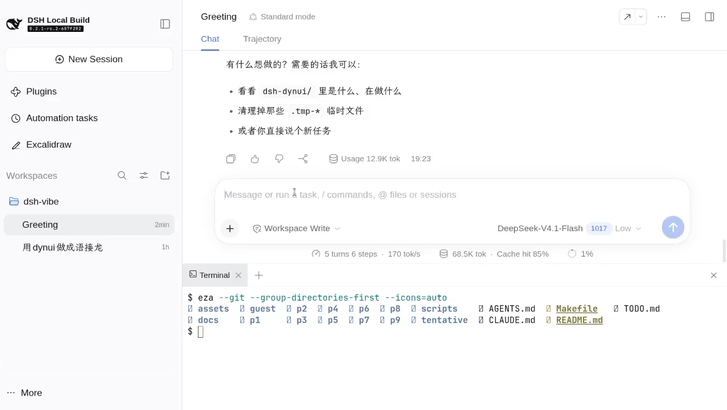
\includegraphics[width=0.84\textwidth]{figures/fig_29_better_sidebar_creator.png}
\caption{社区插件扩展后的 DeepSeek Harness 界面：左侧集成工作区、插件与 Excalidraw 入口，右下角通过 \texttt{dsh-better-sidebar} 嵌入完整的交互式 Terminal、文件树、Git 与 Side Chat\vtag}
\end{figure}
\srcnote{00:57:30--00:57:45}

如图 29 所示，\texttt{dsh-better-sidebar} 完全在插件内部维护了文件浏览器（Files）、Git 状态面板、交互式终端（Terminal）、任务列表与副聊天窗（Side Chat）的 UI 状态，只通过观察主 \texttt{Session} 并绑定到底部和侧边栏插槽，就在不触碰任何底层代码的前提下，把一个极简聊天框变成了堪比 Cursor 的全功能集成开发环境。

\subsection{Creator Mode（创造模式）：让 Agent 在运行中给自己热插拔写插件}

既然人类开发者可以通过“许愿式编程”写插件，那么更进一步：\textbf{为什么不让正在运行的 Agent 直接根据用户的许愿，当场给自己写一个新插件并热加载进宿主系统呢？}——恭喜你，你发明了 DeepSeek Harness 中最令人惊叹的 \textbf{\texttt{Creator Mode}（创造模式，界面标语为“Into the Unknown”）}！

普通模式（Standard Mode）下的 Agent 会话受到严格沙箱限制，只能读写当前工作区目录或执行受控命令；而一旦切换到火力全开的 \textbf{Creator Mode}，系统就向该 Agent 会话授予了操作底层 \textbf{Cordis 插件容器}的特权（如调用 \texttt{cordis.installBundle}）。这意味着：\textbf{Agent 可以在与你对话的过程中，“看见”自己所处的宿主世界，动态编写、编译、挂载甚至卸载它自己的插件！}

主讲教师在课堂现场做了一个即兴实验（当时处于“梁文峰时间”高并发时段，但 DeepSeek-V4.1-Flash 的推理速度依然高达 \textbf{200}～\textbf{250} tok/s）：他在 Creator Mode 下向 Agent 许愿：
\begin{quote}
\textbf{“我对现在的 UI 不太满意，能不能在 Token 消耗旁边放一个超大号的（高达驾驶舱风格）显示面板？”}
\end{quote}
Agent 思考片刻后，自动读取了系统的插件接口规范，编写了一个全新的 UI 插件包，并在界面上弹出高危权限审批请求：\texttt{cordis.installBundle}。当教师点击 \texttt{Allow} 授权的瞬间，无需重启服务、甚至无需刷新页面，右下角状态栏旁立刻热加载出了一个带霓虹仪表盘动效的“高达驾驶舱主监视器（\texttt{MAIN MONITOR // TOKEN ONLINE}）”（见后文图 32 右下角）！这种“系统在运行中根据用户意图实时改造自身”的能力，正是全动态插件生命周期与总线架构释放出的核弹级潜力。

\begin{importantbox}{Creator Mode 的自举本质：突破工具与宿主的静态边界}
在传统的 Coding Agent（如早期 Claude Code 或普通 IDE 插件）中，Agent 的操作对象仅限于“用户的工作区代码文件”，而宿主 IDE 本身的界面与控制逻辑对 Agent 而言是不可触碰的“神圣黑盒”。DeepSeek Harness 的 \textbf{Creator Mode} 则通过将 Cordis 插件容器本身暴露为受控能力，拆除了“被开发的项目”与“正在运行的宿主环境”之间的高墙，实现了运行时自举（Runtime Self-Modifying / Bootstrapping）。
\end{importantbox}

\subsection{那么，代价呢？生态碎片、特征交互与级联压缩失真}

遵循“架构没有免费的午餐”定律，DeepSeek Harness 将状态彻底下放给插件、依靠事件总线解耦的设计，必然也有它无法解决的阴暗面——那就是\textbf{插件间的语义冲突（Semantic Conflicts）与生态碎片化}。

\begin{figure}[H]
\centering
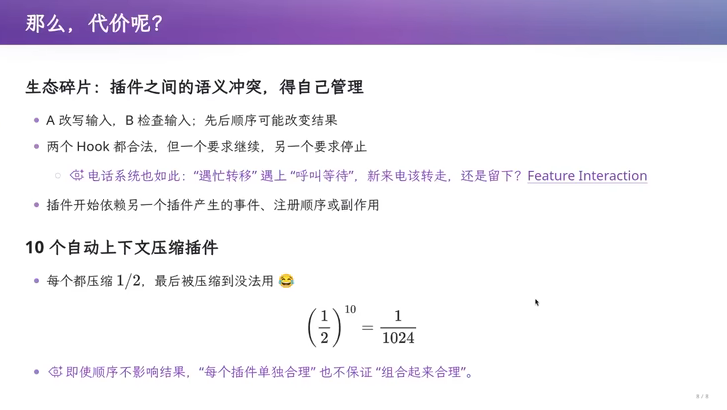
\includegraphics[width=0.84\textwidth]{figures/fig_30_plugin_cost_conflicts.png}
\caption{插件生态的代价：钩子执行顺序引发的语义冲突、电信系统“特征交互（Feature Interaction）”难题，以及 10 个自动上下文压缩插件级联导致 $\left(\frac{1}{2}\right)^{10} = \frac{1}{1024}$ 的信息坍缩\vtag}
\end{figure}
\srcnote{01:03:30--01:03:45}

虽然 TypeScript 编译器保证了每个插件挂载到总线上的事件“类型合法”，但编译器和微内核\textbf{永远无法保证多个插件组合在一起时的“应用语义合理”}：
\begin{enumerate}
    \item \textbf{读写顺序敏感性}：假设插件 A 在 \texttt{pre-step} 中负责改写润色用户输入，插件 B 负责校验用户输入是否合规。到底应该先检查再改写，还是先改写再检查？注册顺序的不同会直接改变系统行为。
    \item \textbf{决策冲突与“特征交互（Feature Interaction）”}：如果两个合法挂载的 Hook 同时介入决策，一个要求“继续执行”，另一个要求“立即停止”，谁说了算？这种难题早在传统程控电话系统时代就曾让电信工程师焦头烂额——著名的\textbf{特征交互问题（Feature Interaction Problem）}：当用户同时开通了“遇忙呼叫转移（Call Forwarding on Busy）”和“呼叫等待（Call Waiting）”两个单独看都完全合理的服务时，一旦通话中来了新电话，系统到底应该把它转走，还是接进来响提示音？
    \item \textbf{级联变换的指数失真}：假设一个自动上下文压缩插件单独工作时非常合理，每次在 \texttt{pre-step} 中把过长的上下文精简压缩为原来的 $\frac{1}{2}$。如果一位不明真相的用户在插件市场里一口气安装了 \textbf{10} 个不同作者写的自动上下文压缩插件，且它们互不知情地串联在同一个 \texttt{pre-step} 钩子链上，那么经过 10 次级联压缩后，原始上下文剩余的信息比例 $R$ 将衰减为：
    \[
        R = \left(\frac{1}{2}\right)^{10} = \frac{1}{1024}
    \]
    式中，$\frac{1}{2}$ 为单个压缩插件的单步保留率，$10$ 为串联挂载的同类插件个数，$R = \frac{1}{1024}$ 为最终送入大模型的有效上下文比例——此时上下文已被浓缩成毫无意义的残渣！
\end{enumerate}

\begin{warningbox}{每个插件单独合理 $\neq$ 组合起来合理}
插件化只能消除模块耦合带来的\textbf{偶然复杂性}，却无法消灭多业务规则交织带来的\textbf{本质复杂性}。当多个插件必须协调彼此的意图（例如共享压缩配额或协商锁）时，它们往往不得不额外引入一个共享的“黑板（Blackboard）”状态区，而这又会在局部造成一定程度的抽象泄漏。
\end{warningbox}

尽管存在上述代价，从软件维护与开源生态的角度看，DeepSeek Harness 的策略依然极其高明：正如创新管理学者埃里克$\cdot$冯$\cdot$希佩尔（Eric von Hippel，\textbf{2001}）提出的\textbf{“用户创新工具箱（User Toolkits for Innovation）”}理论所言，当用户的真实需求高度个性化且模糊多变时，与其让官方产品经理反复调研、排期开发，不如官方只交付一个极简但坚固的内核，把试错和定制留在用户现场，让全球开发者用近乎零成本的 Vibe Coding 自行长出万千生态。

\subsection{本章小结}

本节展示了 DeepSeek Harness 插件生态从零槽位 TUI、\texttt{dsh-better-sidebar} 到运行时自举热插拔插件的 \texttt{Creator Mode} 的强大表现，同时定量剖析了多插件串联引发的 $\left(\frac{1}{2}\right)^{10} = \frac{1}{1024}$ 级联失真与特征交互冲突，阐明了开源微内核“把试错留在用户现场”的生态演化哲学。

\section{杀手级应用方向：大型应用桥接与生成式界面（GenUI）}\label{sec:applications}

在主讲教师看来，目前开源社区用 DeepSeek Harness 搓出来的“高达驾驶舱监控”、“UI 美化小组件”虽然好玩，但多少有些“被带歪了”，还没真正发挥出这条事件总线的最大杀伤力。如果由具备深厚系统架构经验的开发者来主导，DeepSeek Harness 最具颠覆性的两个杀手级应用方向是：\textbf{方向一，传统大型应用（SuperApp）的原生 AI 增强}；\textbf{方向二，双向交互的生成式用户界面（GenUI）}。

\subsection{方向一：大型 App 的 AI 增强——三步极薄桥接与 Excalidraw 现场演示}

想想我们日常使用的 WPS Office、Blender、AutoCAD 或大型工业软件（SuperApp）。目前市面上许多 AI 办公产品（如 Kimi、WorkBuddy 的 PPT 生成器）走了一条非常笨重的路线：AI 团队自己从头手搓一个简陋的网页版 PPT 编辑器，功能可能连成熟 Office 软件的十分之一都不到。为什么不反过来思考：\textbf{如何用最小的代价，把一个现成的大型成熟应用直接接入 DeepSeek Harness 的整个插件生态？}

主讲教师指出，任何拥有内部对象模型的 SuperApp（就像早年 Office 通过 VBA 暴露文档对象一样），只需要接入一个\textbf{极薄的三步桥接层（Bridge）}：
\begin{enumerate}
    \item \textbf{锁定对象（Lock Objects）}：在应用界面上框选一部分对象（如幻灯片的第 2 页、画布上的某几个图形元素）并将其加锁，防止 AI 处理期间人类并发修改引发冲突，而画布其余未加锁区域人类仍可照常自由编辑。
    \item \textbf{序列化交接（Serialize / Handoff Objects to Bus）}：将锁定对象的结构化表示通过总线送入 DeepSeek Harness 的模型上下文。
    \item \textbf{结果回写替换（Apply Back to SuperApp）}：模型调用总线上挂载的各种工具、个人数据库插件完成修改后，将新对象反序列化替换回原应用并释放锁。
\end{enumerate}

为了证明这一模式的可行性，主讲教师在课前仅花了 \textbf{5分钟} 时间，用许愿式编程（Vibe Coding）将著名开源手绘白板应用 \textbf{Excalidraw} 包装成了 DeepSeek Harness 的一个宿主插件（\texttt{dsh-excalidraw}），并在课堂上做了现场实时演示：

\begin{figure}[H]
\centering
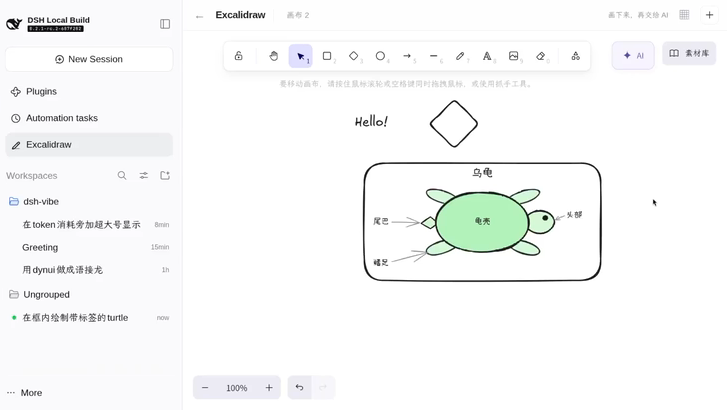
\includegraphics[width=0.84\textwidth]{figures/fig_31_superapp_excalidraw.png}
\caption{大型应用 AI 增强现场演示：将开源白板 Excalidraw 通过极薄桥接层接入 DeepSeek Harness，框选局部区域后由 AI 自动绘制并标注出由几何图元拼成的“乌龟”\vtag}
\end{figure}
\srcnote{01:11:00--01:11:15}

在演示中，教师先在 Excalidraw 画布上方随手画了一个菱形并写下 \texttt{Hello!}，接着在下方拉出一个矩形选框，点击右上角的“\texttt{AI}”按钮发出指令：“\textbf{在框内绘制带标签的 turtle（致敬 Logo 语言小海龟）}”。此时：
\begin{itemize}
    \item 选框区域在前端被标记为锁定态（Locked），而在 AI 后台思考绘图的 27 秒内，教师依然可以在画布其他位置自由拖拽编辑；
    \item 随后，DeepSeek-V4.1-Flash 模型生成的标准 Excalidraw 图元直接落入框内，精准拼出了一只带浅绿色椭圆“\textbf{龟壳}”、右侧“\textbf{头部}”与眼睛、四片“\textbf{鳍足}”和三角形“\textbf{尾巴}”且带箭头文字标注的乌龟！
    \item 更美妙的是，生成出来的乌龟不是一张死板的位图图片，而是原生的 Excalidraw 矢量对象——如果不喜欢龟壳的颜色或某条腿的位置，用户可以随时点中它二次编辑或删除！
\end{itemize}

想象一下，如果一款开源办公套件（不妨叫“XPS”）哪怕只有 WPS 七到八成（70\%～80\%）的基础排版功能，
但通过这套协议原生接入了你的 DeepSeek Harness：当你要填写一份令人抓狂的科研申报表格（例如要求填报“从 \textbf{2021年} 到现在发表的所有论文、指导学生与项目经费明细”）时，你不再需要让 Codex 或 Computer Use 笨拙地不断截屏、识别坐标、模拟鼠标点击，而是由表格应用把“待填单元格对象”往总线上一丢，总线上挂载的“个人学术数据库插件”瞬间检索出你自 \textbf{2021年} 以来的全套论文 BibTeX 与项目记录，零截图、零多余 Token 消耗地一把将整张复杂表格精准填完！

\begin{knowledgebox}{结构化对象总线桥接 vs. 视觉 GUI 模拟（Computer Use）}
为什么通过总线桥接操作应用内部对象（如 Excalidraw 图元或表格单元格）远优于基于截屏点击的 Computer Use？
\begin{itemize}
    \item \textbf{Token 与延迟降低两个数量级}：无需反复传输高分辨率屏幕截图与坐标推理，直接传递紧凑的 JSON 对象树。
    \item \textbf{支持细粒度并发与非阻塞协作}：只锁定用户框选的局部对象 ID，人类用户可同时在同一画布或文档的其余区域继续编辑，不会像 GUI 模拟那样抢占整个系统的鼠标与键盘焦点。
\end{itemize}
\end{knowledgebox}

\subsection{方向二：生成式用户界面（GenUI）——卡片与上下文的双向通道}

第二个极具想象力的方向是 \textbf{Generative UI（生成式用户界面，简称 GenUI）}。传统的聊天界面里，模型只能输出静态的 Markdown 文本；但如果我们在 DeepSeek Harness 总线上做一个简单的约定：
\begin{enumerate}
    \item \textbf{模型输出交互卡片（Model $\to$ UI Card）}：通过 \texttt{systemPrompt} 向模型注入一段仅 \textbf{1.5KB} 的轻量级协议说明，允许模型在回复中输出带有特定类名标记（例如 \texttt{dsh-dynui} 容器节点）的 HTML + JavaScript 交互卡片，由前端插件捕获并渲染在界面插槽中。
    \item \textbf{卡片动作回注上下文（UI Card $\to$ Model Context）}：卡片内的 JavaScript 代码可以通过受控桥接函数（如触发 \texttt{session.prompt} 或向 Event Bus 发送事件），将用户在卡片上的鼠标点击、落子坐标和当前组件状态直接格式化成精确的状态字符串，重新注入回大模型的上下文中，触发模型下一轮思考与界面更新！
\end{enumerate}

主讲教师同样只花了 \textbf{5分钟} Vibe 出了这个名为 \textbf{\texttt{dsh-dynui}} 的动态 UI 插件，并在课堂上演示了两个生动的交互应用：
\begin{itemize}
    \item \textbf{交互式成语接龙卡片}：模型生成一个带输入框和按钮的成语接龙游戏卡片。当用户点击“以‘惊弓之鸟’开局”按钮时，卡片内的 JS 自动拼接出一句结构化提示词注入会话，模型接出“鸟语花香 $\to$ 香火不绝 $\to$ 绝处逢生”，并实时生成更新了历史记录栈的新卡片。
    \item \textbf{和 DeepSeek 下五子棋（Gomoku）}：教师直接向 Agent 许愿：“\textbf{用 dynui 做一个五子棋，要求五子棋的状态在 UI 里，但所有下棋落子都是模型思考以后做的。}”
\end{itemize}

\begin{figure}[H]
\centering
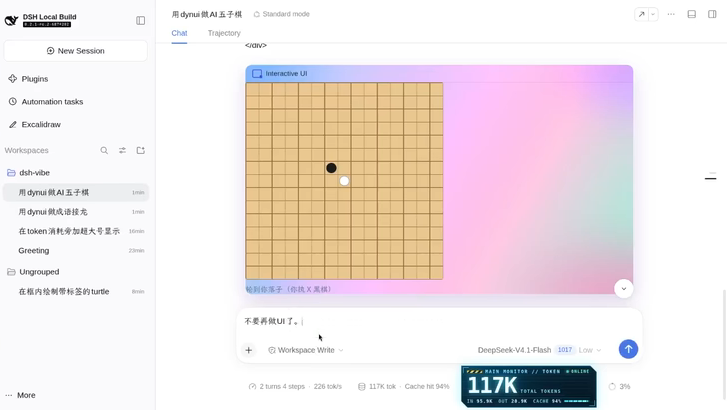
\includegraphics[width=0.84\textwidth]{figures/fig_32_genui_gomoku_contracts.png}
\caption{GenUI 双向交互演示：模型动态生成 HTML+JS 五子棋盘卡片（人类点击棋盘落黑子，JS 自动将棋局状态回注上下文驱动模型落白子），右下角同时展示 Creator Mode 热生成的 \texttt{117K} Token 驾驶舱监视器\vtag}
\end{figure}
\srcnote{01:18:45--01:19:00}

如图 32 所示，模型当场生成了一个 $15 \times 15$ 的木纹五子棋盘卡片。人类玩家只需用鼠标在棋盘交叉点上轻轻一点落下黑子，卡片中的 JavaScript 就会自动校验落子合法性，并将当前棋盘坐标状态回传给 DeepSeek 模型；模型经过简短思考后计算出应对策略，落下白子并刷新棋盘卡片！
\begin{importantbox}{GenUI 的核心设计哲学：代码管渲染校验，模型管意图决策}
在五子棋这类交互应用中，如果让纯文本大模型用自然语言去画 ASCII 棋盘或判断五子连珠，既浪费 Token 又容易出现坐标幻觉；而 \textbf{GenUI 建立的双向通道实现了完美分工：把确定性的界面渲染、点击事件捕获与规则校验交给卡片里的 JavaScript 代码，用结构化状态精确表达动作，而让大语言模型专注于策略思考与意图决策。}虽然课堂 5 分钟写出的原型还是每次整卡重绘（未来完全可以演进为增量 DOM Patch 协议），但这正如当年初次看到 GPT-3.5 虽然从 50 数到 100 还会卡壳重复，却已让人瞥见通往未来的无限可能。
\end{importantbox}

\subsection{本章小结}

本节展示了 DeepSeek Harness 在两个前沿方向上的突破性应用：一是通过“锁定对象 + 序列化交接 + 结果回写”三步极薄桥接层赋能 Excalidraw 等大型传统应用（SuperApp）；二是通过 1.5KB 协议说明与 \texttt{dsh-dynui} 建立 HTML+JS 卡片与模型上下文的双向通道，实现成语接龙与 AI 五子棋等生成式界面（GenUI）。

\section{源码级架构复盘与总结延伸}\label{sec:contracts}

在演示完令人眼花缭乱的插件生态与杀手级应用后，课程最后十分钟回到了严谨的系统工程视角：主讲教师开启了一个终端 Coding Agent，让它直接阅读本地的 DeepSeek Harness 源码仓库以及刚刚花 5 分钟 Vibe 出来的 \texttt{dsh-excalidraw} 与 \texttt{dsh-dynui} 插件源码，生成了一份刀刀见血的\textbf{源码级架构与边界审计报告}。

\subsection{DeepSeek Harness 的五条核心源码契约}

通过对 \texttt{packages/} 下核心模块（\texttt{core}、\texttt{cordis}、\texttt{agent}、\texttt{session}、\texttt{tools}、\texttt{web} 等）的走读，我们可以将 DeepSeek Harness 的底层架构精炼为\textbf{五条不可违背的核心契约}：

\begin{table}[H]
\centering
\small
\begin{tabular}{p{0.8cm}p{3.2cm}p{4.8cm}p{5.0cm}}
\toprule
\textbf{编号} & \textbf{契约名称} & \textbf{源码级机制与约束} & \textbf{解决的工程问题} \\
\midrule
契约 1 & \textbf{Append-only 事实流契约} & \texttt{Session} 仅暴露 \texttt{append()} 与事件流读取，严禁原地修改或删除历史条目；流式输出通过末尾临时的 \texttt{Open Entry} 承载 & 保证全局唯一事实源（Ground Truth），天然支持崩溃恢复、重放审计与跨端同步 \\
契约 2 & \textbf{Projection 只读派生契约} & 模型上下文（\texttt{deriveMessages}）与业务视图（\texttt{sessionProjections}）均为事件流上的纯函数折叠，投影层不持有独立权威状态 & 允许同一份会话历史同时投影为人类 Chat 界面、开发者 Trajectory 面板或 VS Code 工作台 \\
契约 3 & \textbf{Pre-step 洋葱圈拦截契约} & \texttt{agent/pre-step} 采用 \texttt{async (payload, next) => ...} 中间件链，调用 \texttt{next()} 才放行后续环节 & 在不侵入主循环的前提下，统一实现上下文动态改写、自动压缩、预算熔断与执行拦截 \\
契约 4 & \textbf{Scope 隔离与权限单调求交契约} & 基于 Cordis 的 \texttt{Scope} 追踪插件生命周期；工具权限控制（\texttt{tools.guard()}）遵循\textbf{单调拒绝（Monotonic Deny）}原则——下游只能收紧权限，绝不能把上游的 \texttt{deny} 翻回 \texttt{allow} & 确保插件卸载时副作用全回收，且编译期/运行期阻止恶意或失控插件越权清空或篡改全局工具集 \\
契约 5 & \textbf{Slots 界面解耦契约} & Web 前端仅定义命名挂载点（\texttt{slots}），核心逻辑不依赖任何具体 DOM 组件 & 使 Web UI 组件热插拔与无槽位的纯命令行 \texttt{TUI} 能够无缝共存于同一套内核之上 \\
\bottomrule
\end{tabular}
\caption{DeepSeek Harness 源码级提炼的五条核心架构契约}
\end{table}

\subsection{对 \texttt{dsh-excalidraw} 实现的真实工程取舍审视}

有了这五条标准契约作为尺子，我们再来审视课堂上花 5 分钟许愿写出来的 \texttt{dsh-excalidraw} 插件源码，就会发现快速原型为了“一把跑通”在架构上做了哪些真实的妥协与取舍：

\begin{figure}[H]
\centering
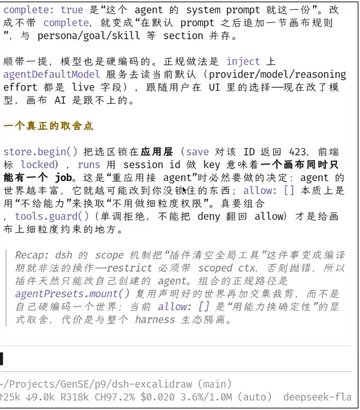
\includegraphics[width=0.52\textwidth]{figures/fig_33_five_contracts_audit.png}
\caption{课堂终端源码审计：剖析 \texttt{dsh-excalidraw} 插件中 \texttt{complete: true} 提示词覆盖、\texttt{store.begin()} 返回 HTTP \texttt{423} 选区锁以及 \texttt{allow: []} 与 \texttt{tools.guard()} 权限裁剪之间的架构取舍\vtag}
\end{figure}
\srcnote{01:27:00--01:27:15}

如图 33 终端输出所示（注意底栏显示该次深度源码分析的缓存命中率高达 \texttt{CH97.2\%}，花费仅 \texttt{\$0.020}）：
\begin{enumerate}
    \item \textbf{\texttt{complete: true} 独占系统提示词 vs. 追加 Section 并存}：5 分钟 Vibe 出的画布插件在创建内部推理会话时传入了 \texttt{complete: true}，这意味着“这个 Agent 的 System Prompt 就只有画布规则这一份”，从而粗暴屏蔽了宿主的 persona、goal、skill 等其他提示词片段；如果改成正规的不带 \texttt{complete} 的追加模式，画布 AI 就能与其他技能插件并存协作。同理，原型中硬编码了模型名称，正规做法应当注入 \texttt{agentDefaultModel} 服务去读取用户在 UI 里实时选择的 live 字段。
    \item \textbf{\texttt{store.begin()} 应用层选区锁与 HTTP \texttt{423 Locked}}：为了防止 AI 绘图时用户并发修改同一选区，插件通过 \texttt{store.begin()} 将选区 ID 锁在应用层（此时前端标为 \texttt{locked}，若并发保存该 ID 则服务端返回 HTTP 状态码 \textbf{\texttt{423}}），且 \texttt{runs} 字典以 \texttt{session id} 作为 Key，意味着\textbf{同一张画布同时只能跑一个 AI Job}。
    \item \textbf{\texttt{allow: []} 孤岛模式 vs. \texttt{agentPresets.mount()} 生态组合}：这是“重型应用接入 Agent”时最深刻的一个架构取舍点——\textbf{Agent 能调用的外部世界越丰富，它就越有可能误改到你没锁住的东西。}为了省去细粒度权限控制，5 分钟原型直接设置了 \texttt{allow: []}（清空所有外部工具，只让模型纯靠推理吐出画布 JSON），这本质上是\textbf{“用不给能力来换取确定性，代价是与整个 Harness 工具生态隔离”}。如果未来要让画布 AI 既能调外部数据库查论文、又绝不破坏画布外的文件，正规路径应当是通过 \texttt{agentPresets.mount()} 复用声明好的世界，再用 \texttt{tools.guard()} 做单调拒绝（Monotonic Deny）的交集裁剪。
\end{enumerate}

\begin{warningbox}{权限设计的单调拒绝（Monotonic Deny）铁律}
在多插件协同的微内核架构中，为什么 \texttt{tools.guard()} 必须强制实行“单调求交（只能把 \texttt{allow} 缩减为 \texttt{deny}，绝不允许下游把上游已判定的 \texttt{deny} 翻转为 \texttt{allow}）”？因为如果允许后挂载的业务插件随意覆写全局白名单，任何一个疏忽或恶意的第三方 UI 小插件都能静默解除沙箱限制并获取宿主机 Shell 的完全控制权。单调拒绝契约在架构层面保证了安全边界的不可逆收敛。
\end{warningbox}

\subsection{核心要点回顾与延伸思考}

至此，我们完成了对 DeepSeek Harness 第一部分的完整剖析。回顾整堂课的脉络：
\begin{itemize}
    \item \textbf{从需求看本质复杂性}：150 行的 Mini-Agent 可以凭一句话生成南大仙林校区三维地图，但高铁上的一次断网就暴露出会话持久化、指数退避重试、非幂等副作用核实等无法逃避的本质复杂性；而 Grok Bot 式的交互范式突变，更是直接宣判了僵化耦合架构的死刑。
    \item \textbf{从历史看架构权衡}：无论是操作系统进程、LAMP、Event Sourcing，还是 OSDI 2004 的 MapReduce 与后来的 Spark、Flink，架构永远是在“受限（规矩）”与“自由”之间做取舍。当底层假设（如单机可靠、离线批处理、写代码极其昂贵）改变时，旧架构就会因抽象泄漏而沦为阻力。
    \item \textbf{从 DeepSeek Harness 看 Agent 时代的微内核答案}：通过 \texttt{Everything Is a Plugin}（Cordis 生命周期与副作用自动回收）与 \texttt{Session = list[Event]} 事件溯源世界模型，配合 5 个极简总线原语，\texttt{dsh} 让官方内核保持如白板般精简，同时支撑起 \texttt{dsh-bot}、\texttt{dsh-better-sidebar}、\texttt{Creator Mode} 热插拔、大型应用三步桥接与 GenUI 双向交互卡片等无限可能。正如主讲教师在课末透露的，他们团队正在更底层研发的保密项目 \textbf{AgentOS} 同样秉持 \texttt{Everything Is a Plugin} 理念，并在操作系统层与 DeepSeek Harness 形成上下呼应。下一讲（DeepSeek Harness (2)），我们将进一步深入 DeepSeek Harness 源码仓库内部，剖析其 Agent-Native 开发流程与自动化 CI/CD 体系。
\end{itemize}

\begin{knowledgebox}{课后自检与动手思考题}
\begin{enumerate}
    \item \textbf{概念辨析}：为什么说在 Agent 工具调用中，“客户端没有收到工具返回结果”绝不等于“工具没有执行”？如果让你为 Mini-Agent 的 \texttt{run\_bash} 增加断点恢复机制，你会如何区分安全重放命令与危险副作用命令？
    \item \textbf{API 设计理解}：请对比 DeepSeek Harness 中 \texttt{session/event} 与 \texttt{agent/pre-step} 两个事件监听点的机制差异。为什么上下文自动压缩插件和权限审批插件必须挂载在 \texttt{agent/pre-step} 而不是 \texttt{session/event} 上？
    \item \textbf{架构设计实践}：假设你要把自己常用的笔记软件或 PDF 阅读器作为一个 SuperApp 接入 DeepSeek Harness，请按照本讲提出的“锁定对象 $\to$ 序列化交接 $\to$ 结果回写”三步法，设计该桥接插件所需的最小 JSON 协议与锁粒度。
\end{enumerate}
\end{knowledgebox}

\end{document}
